\documentclass[10.5pt
%,draft
]{article}

\usepackage{ctex}
\usepackage{amsmath}
\usepackage{graphicx}
\usepackage{epstopdf}
\usepackage{tikz}
\usepackage{psfrag}
\usepackage{natbib}
\usepackage{hyperref}
\usepackage{overpic}
\usepackage{rotating}

\begin{document}

\renewcommand{\refname}{参考文献}
\renewcommand{\figurename}{图}
\renewcommand{\abstractname}{摘要}

\title{磁流体力学数值模拟方法——第二次作业\footnote{2019秋季中国科学技术大学研究生课程《磁流体力学的数值模拟方法》}}


\author{毛东巍\footnote{邮箱: mdw97@mail.ustc.edu.cn  学号: SA19007035}\quad 张建\footnote{邮箱: zj250711@mail.ustc.edu.cn  学号: SA19007060}\quad 钟志辉\footnote{邮箱: zzhustc@mail.ustc.edu.cn  学号: SA19007054}}

\date{%
	\scriptsize%
	%CAS Key Laboratory for Basic Plasma Physics, School of Earth and Space Sciences,
	%\\
	%University of Science and Technology of China, Hefei, Anhui 230026, China
	中国科学院近地空间环境重点实验室, 合肥 230026\\
	中国科学技术大学地球和空间科学学院, 合肥 230026
	%
}

\maketitle

\begin{abstract}
本工作为《磁流体力学的数值模拟方法》课程第二次作业, 讨论一维单一变量双曲型方程(行波方程和Burgers方程)的有限差分数值解法. 对于给定初始条件与边界条件的微分方程, 我们以图形表示数值解的发展变化, 比较不同格式, 网格密度, 时间步长的计算结果, 并结合理论分析讨论各种常用差分格式的特点. 
\end{abstract}

\section{引言}
一维单变量函数的一阶双曲型偏微分方程表示了一个波动的传播发展过程, 在线性方程的情况下,
波的形状不随时间改变, 而在非线性方程的情况下, 一个连续有限振幅的波可能发展成有间断的解, 即激波, 或者从激波(间断)演化为连续的解\citep{Whitham1999}. 在数值求解过程中, 通过研究微分方程的数值计算格式, 格点密度, 时间步长等参数对解的影响, 可以数值分析解的物理特性和讨论格式的可靠性.

\section{行波方程}
考察方程
\begin{align}
& \frac{\partial u}{\partial t} + \frac{\partial u}{\partial x} = 0,
\label{EqnCon}
\end{align}
在初值条件
\begin{align}
& u|_{t=0} = \left\{\begin{array}{ll} 0.0, & x < -0.4, \\
1.0 - |x + 0.3| / 0.1, & -0.4 \le x < -0.2, \\
0.0, & -0.2 \le x < -0.1, \\
1.0 , & -0.1 \le x < 0.0, \\
0.0, & x \ge 0.0
\end{array}\right.
\end{align}
下的数值解. 通过有限差分格式, 讨论该方程的物理解和差分格式数值解的特性.
迎风格式
\begin{align}
u_j^{n+1} = u^n - \frac{\Delta t}{\Delta x} (u_j^n - u_{j-1}^n), \label{EqnUpwind}
\end{align}
下各个时刻方程解如图\ref{fig11}. 对比来看, 使用Euler格式
\begin{align}
u_j^{n+1} = u^n - \frac{\Delta t}{\Delta x} (u_{j+1/2}^n- u_{j-1/2}^n), \label{EqnEuler}
\end{align}
得到的结果出现了不稳定的结果, 且不稳定性随时间快速增长, 说明Euler格式不稳定, 不适用于有间断面的情况; 同时展示了另外两种格式, 即Lax-Wenderhoff格式与Minmod格式结果的对比. 
\begin{figure}[htb]
\centering
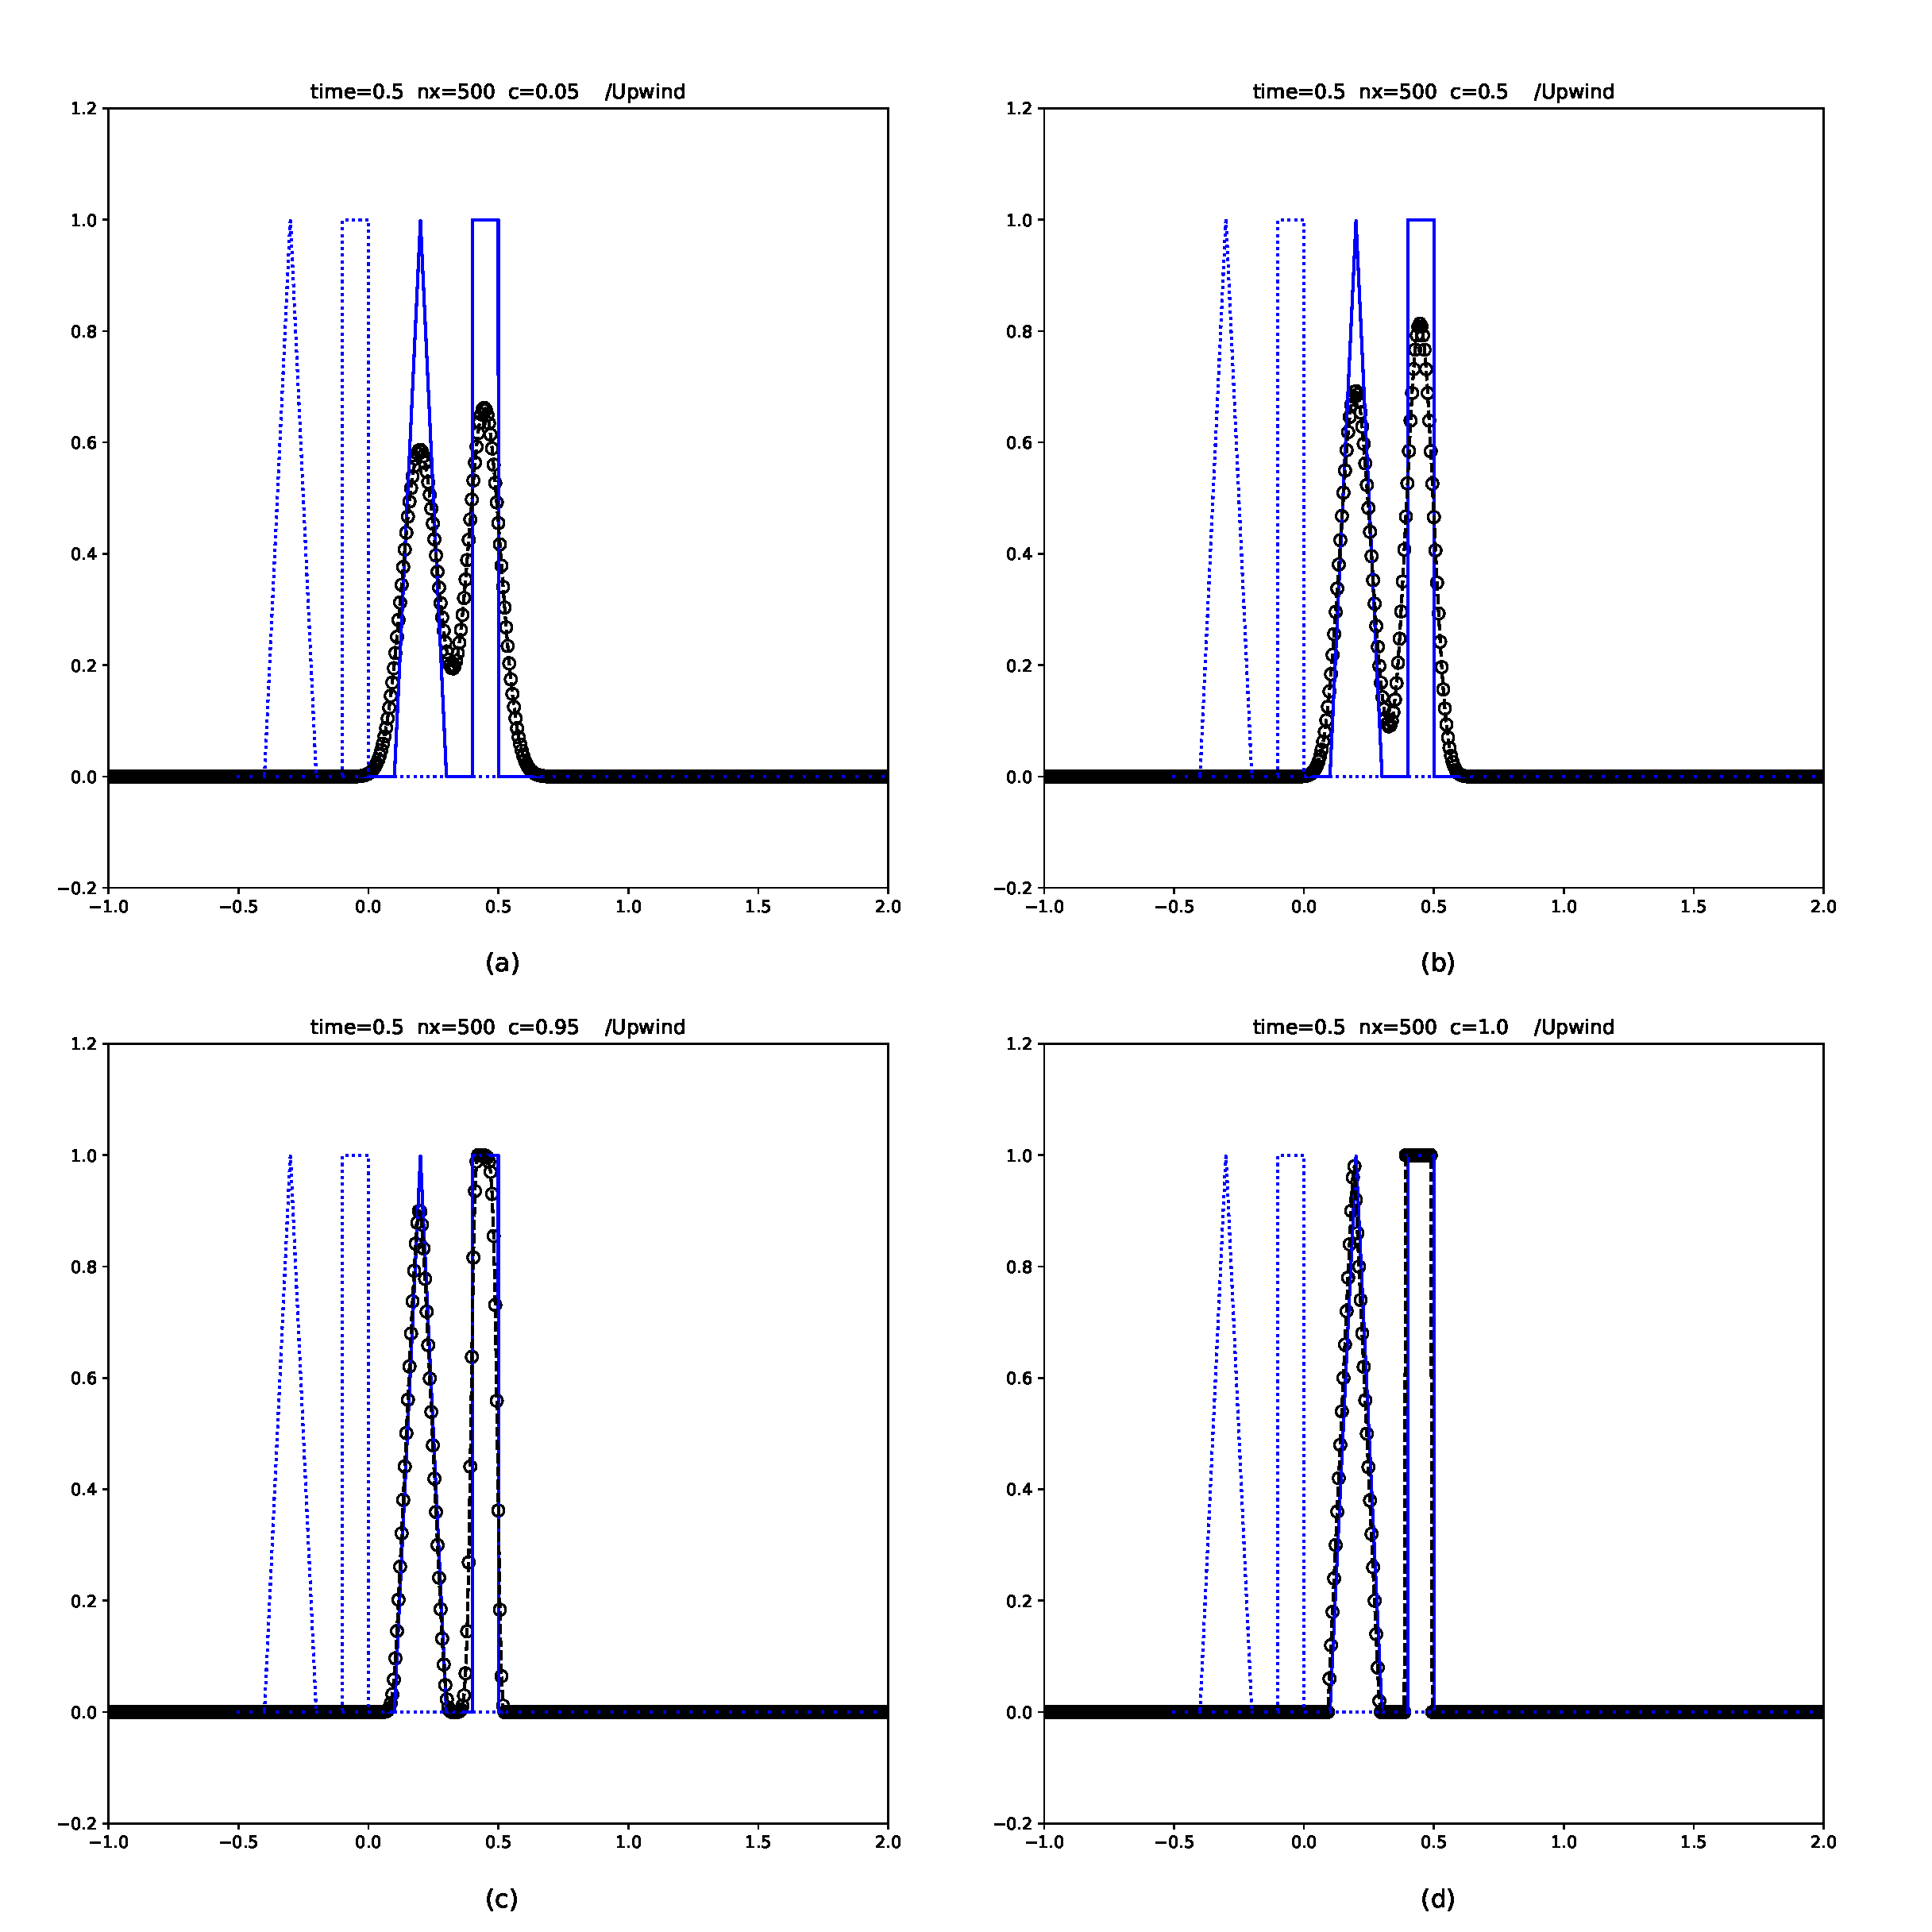
\includegraphics[width=\textwidth]{hw2_1_c.eps}
\caption{方程(\ref{EqnCon})在$t=0.5$时刻的解. 其中虚线表示数值迎风格式的计算结果, 线上的圆圈表示具体网格上的数据. 同一时刻的精确解用实线表示. 作为对照, 初始时刻的值以点线表示, 坐标网格总数为517. (a) 迎风格式, $C = 0.05$, (b)  迎风格式, $C = 0.50$, (c)  迎风格式, $C = 0.95$, (d) 迎风格式, $C = 1.0$, 此时数值结合精确解完全符合, (e) Lax-Wendroff格式, $C=0.95$, 注意其中出现的色散 (上冲和下冲), (f) Minmod格式, $C=0.95$.} \label{fig11}
\end{figure}
\begin{figure}[htb]
	\centering
	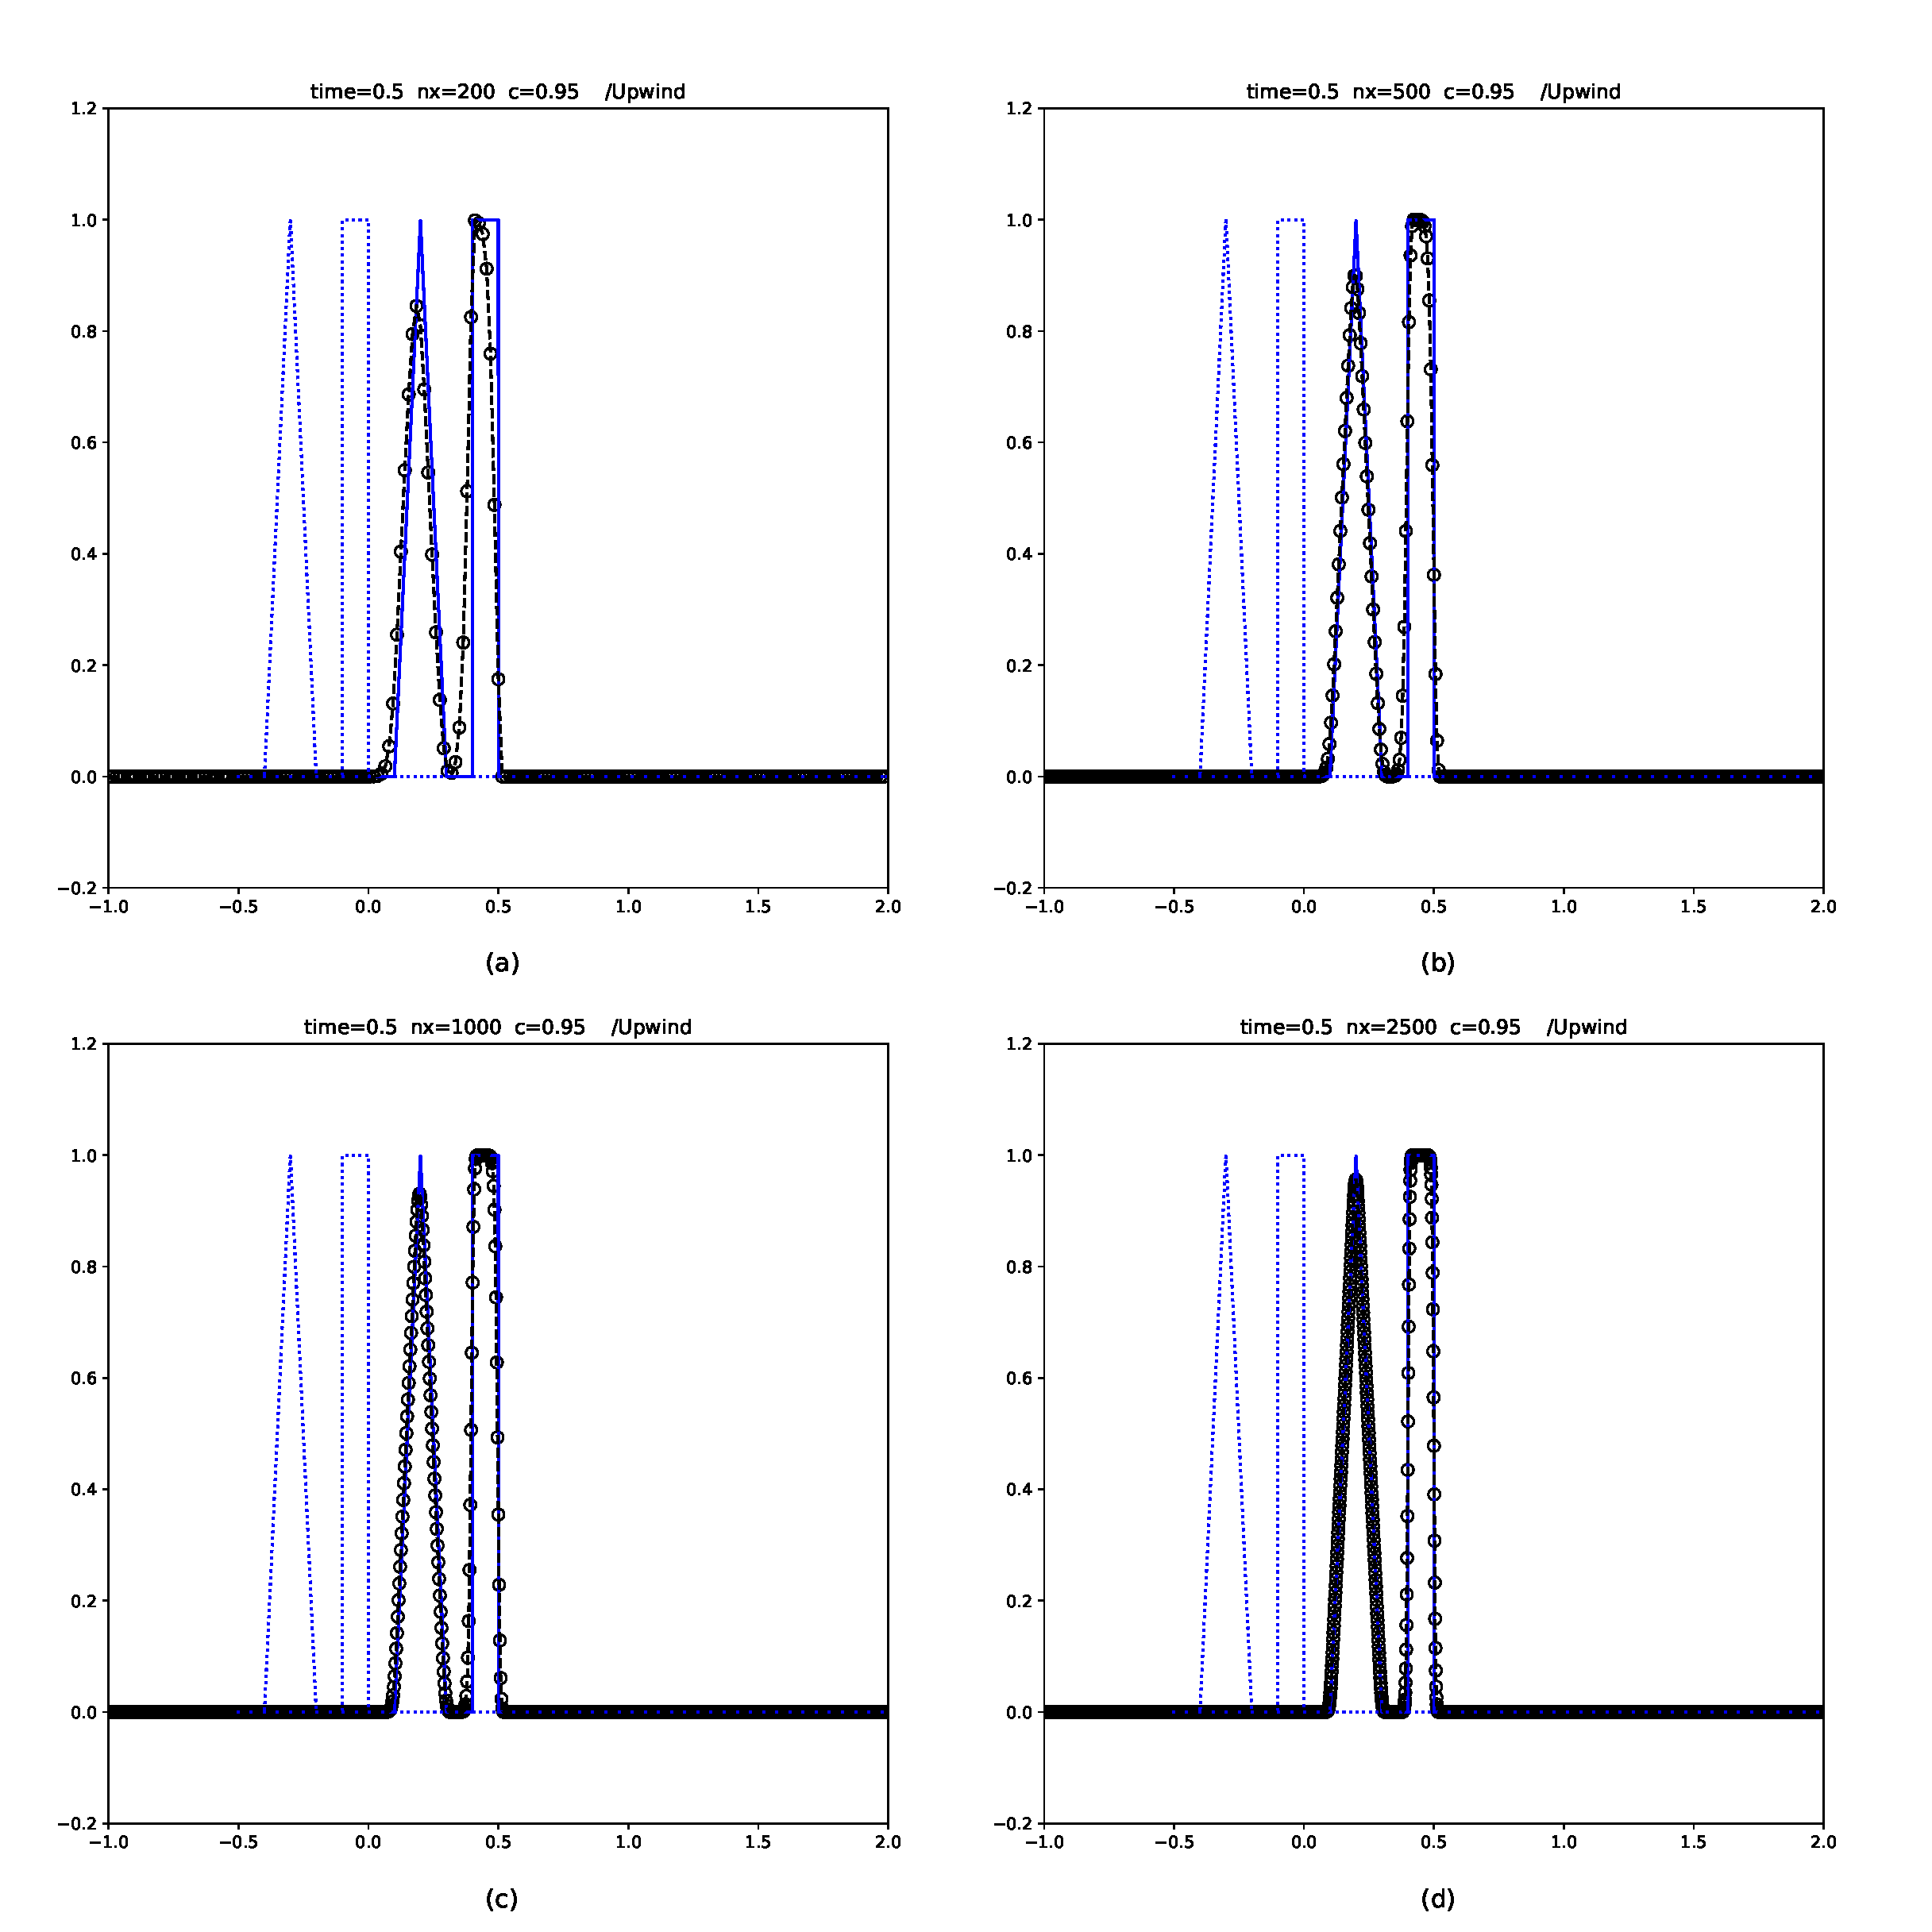
\includegraphics[width=\textwidth]{hw2_1_nx.eps}
	\caption{方程(\ref{EqnCon})在$t=0.5$时刻的解. 其中虚线表示数值迎风格式的计算结果, 线上的圆圈表示具体网格上的数据. 同一时刻的精确解用实线表示. 作为对照, 初始时刻的值以点线表示, Courant系数$C = 0.95$. (a) 迎风格式, $nx = 200$, (b)  迎风格式, $nx = 500$, (c)  迎风格式, $nx = 1000$, (d) 迎风格式, $nx = 2500$.}  \label{fig12}
\end{figure}
\begin{figure}[htb]
	\centering
	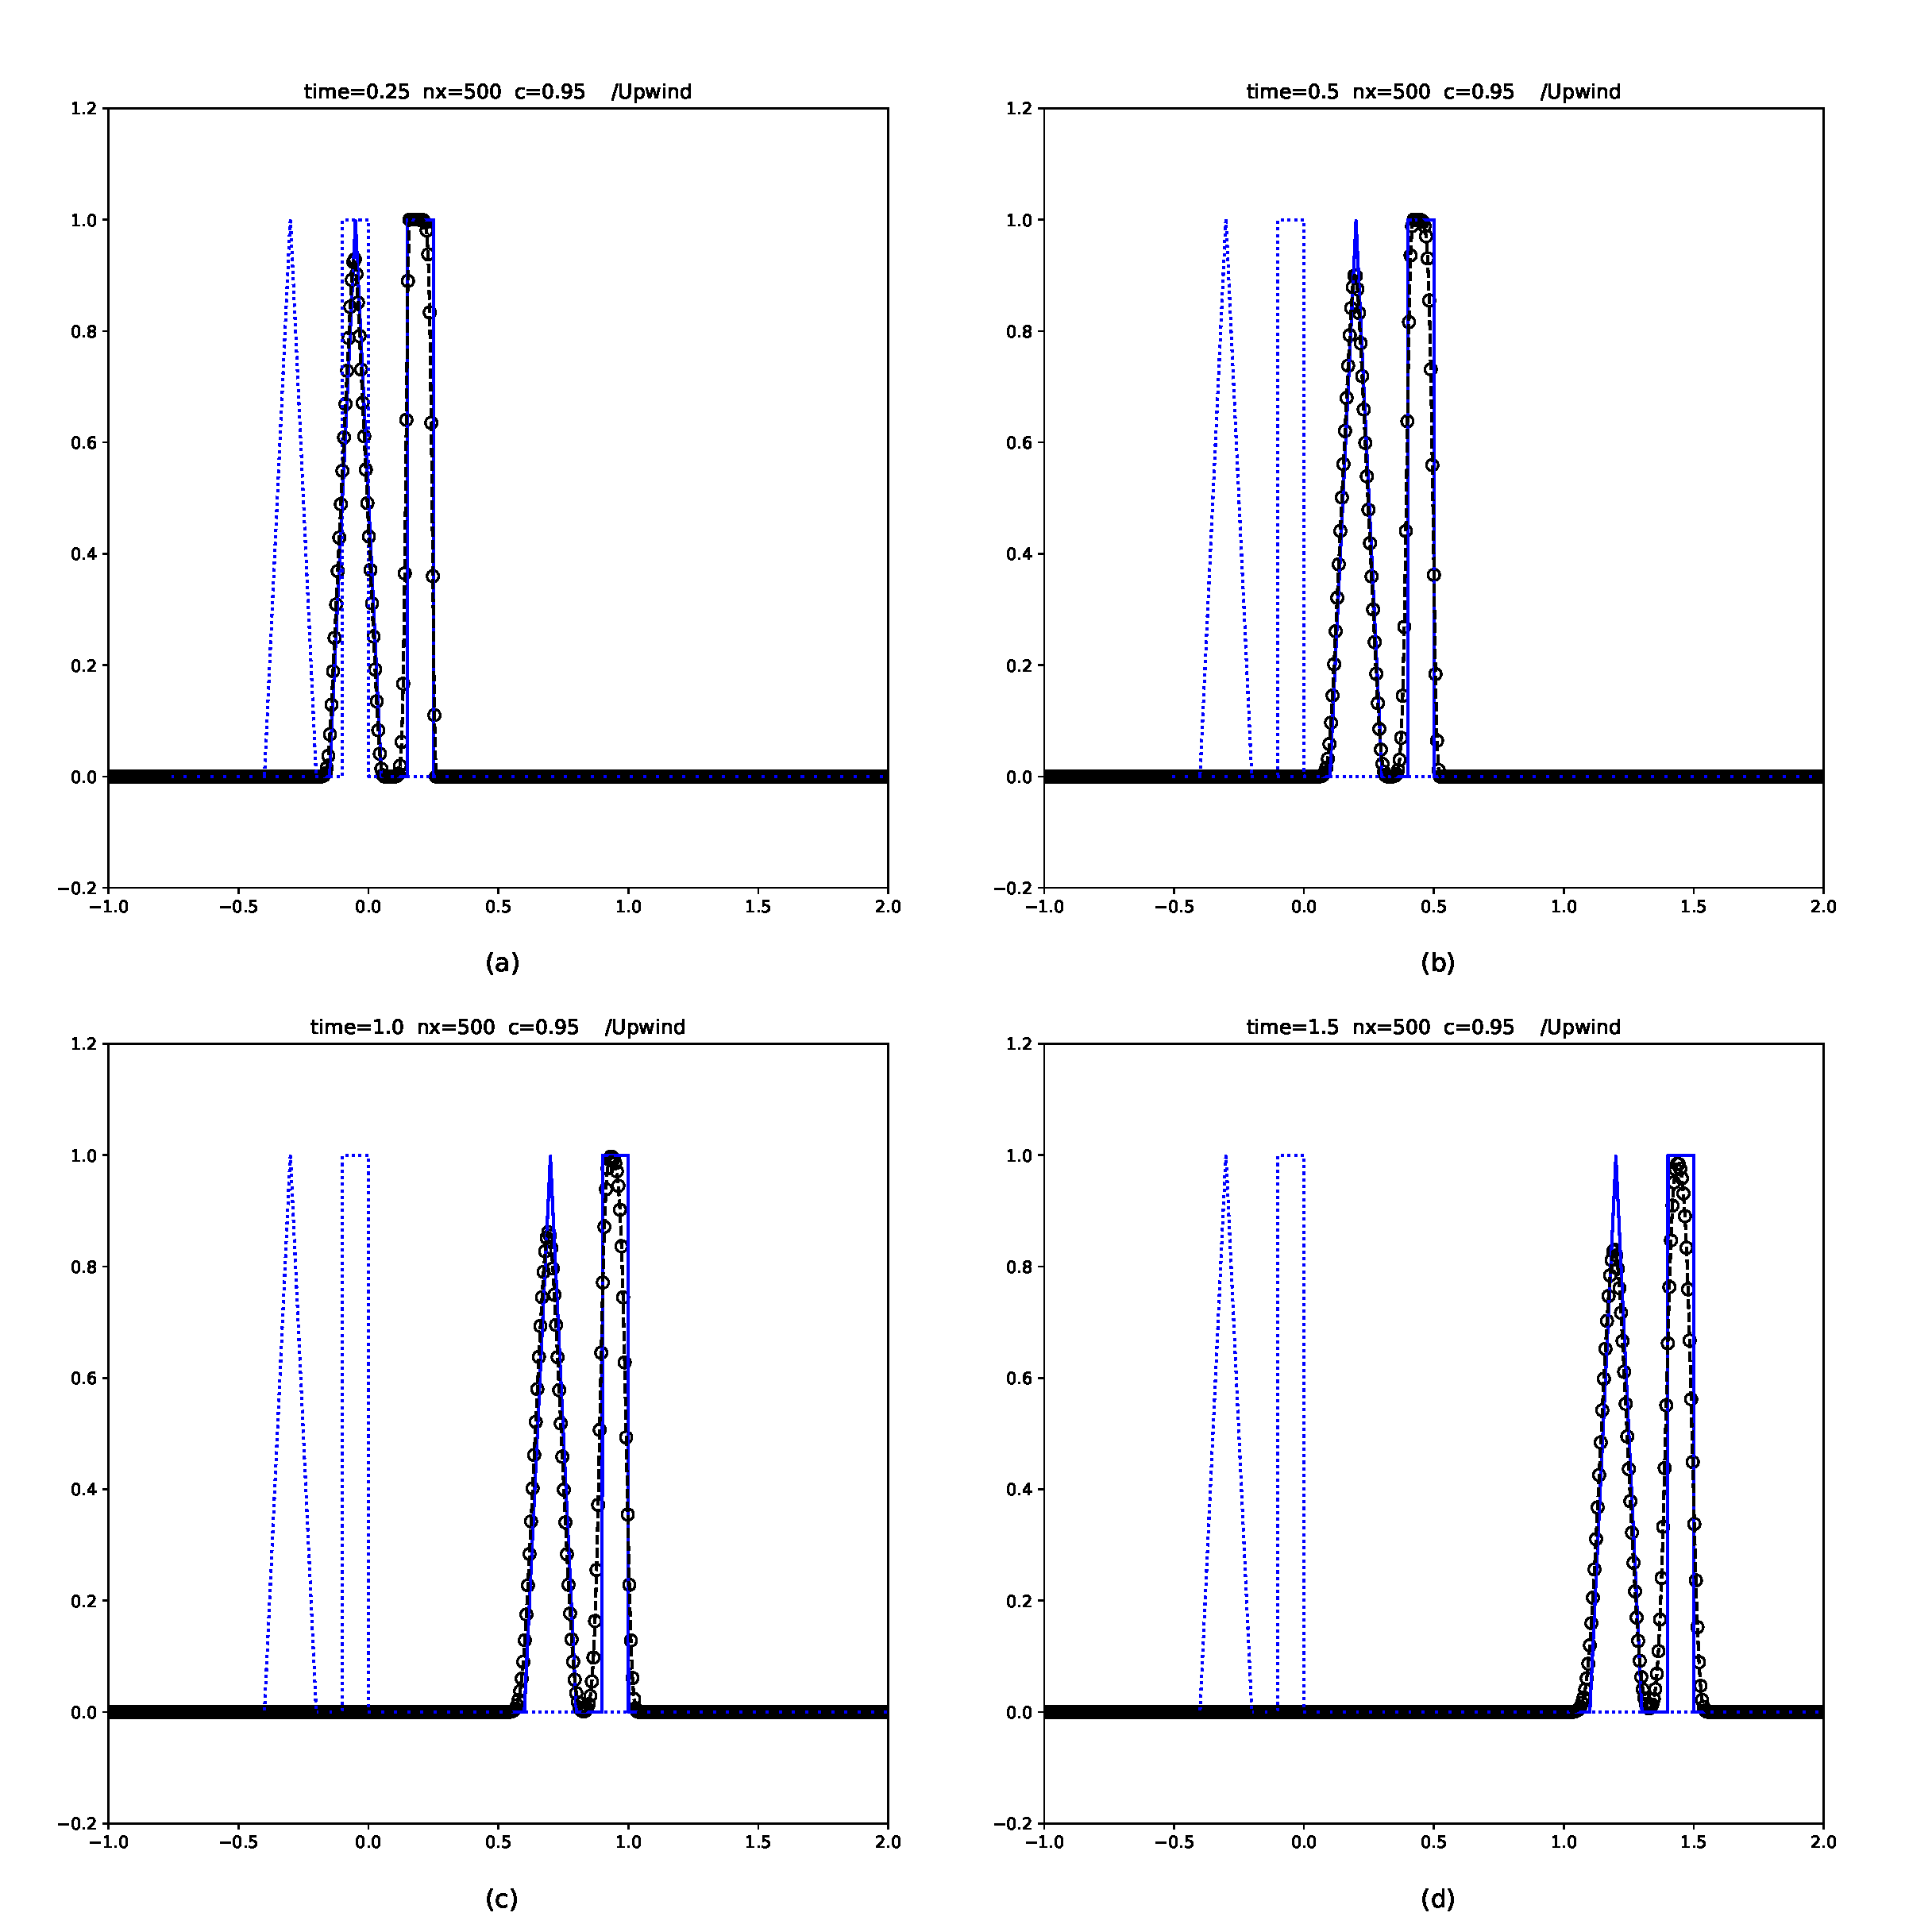
\includegraphics[width=\textwidth]{hw2_1_time.eps}
	\caption{方程(\ref{EqnCon})在不同时刻的解. 其中虚线表示数值迎风格式的计算结果, 线上的圆圈表示具体网格上的数据. 同一时刻的精确解用实线表示. 作为对照, 初始时刻的值以点线表示, 坐标网格总数为500, $C = 0.95$. (a) 迎风格式, $t = 0.25$, (b)  迎风格式, $t = 0.50$, (c)  迎风格式, $t = 1.0$, (d) 迎风格式, $t = 1.5$.}  \label{fig13}
\end{figure}
\begin{figure}[htb]
	\centering
	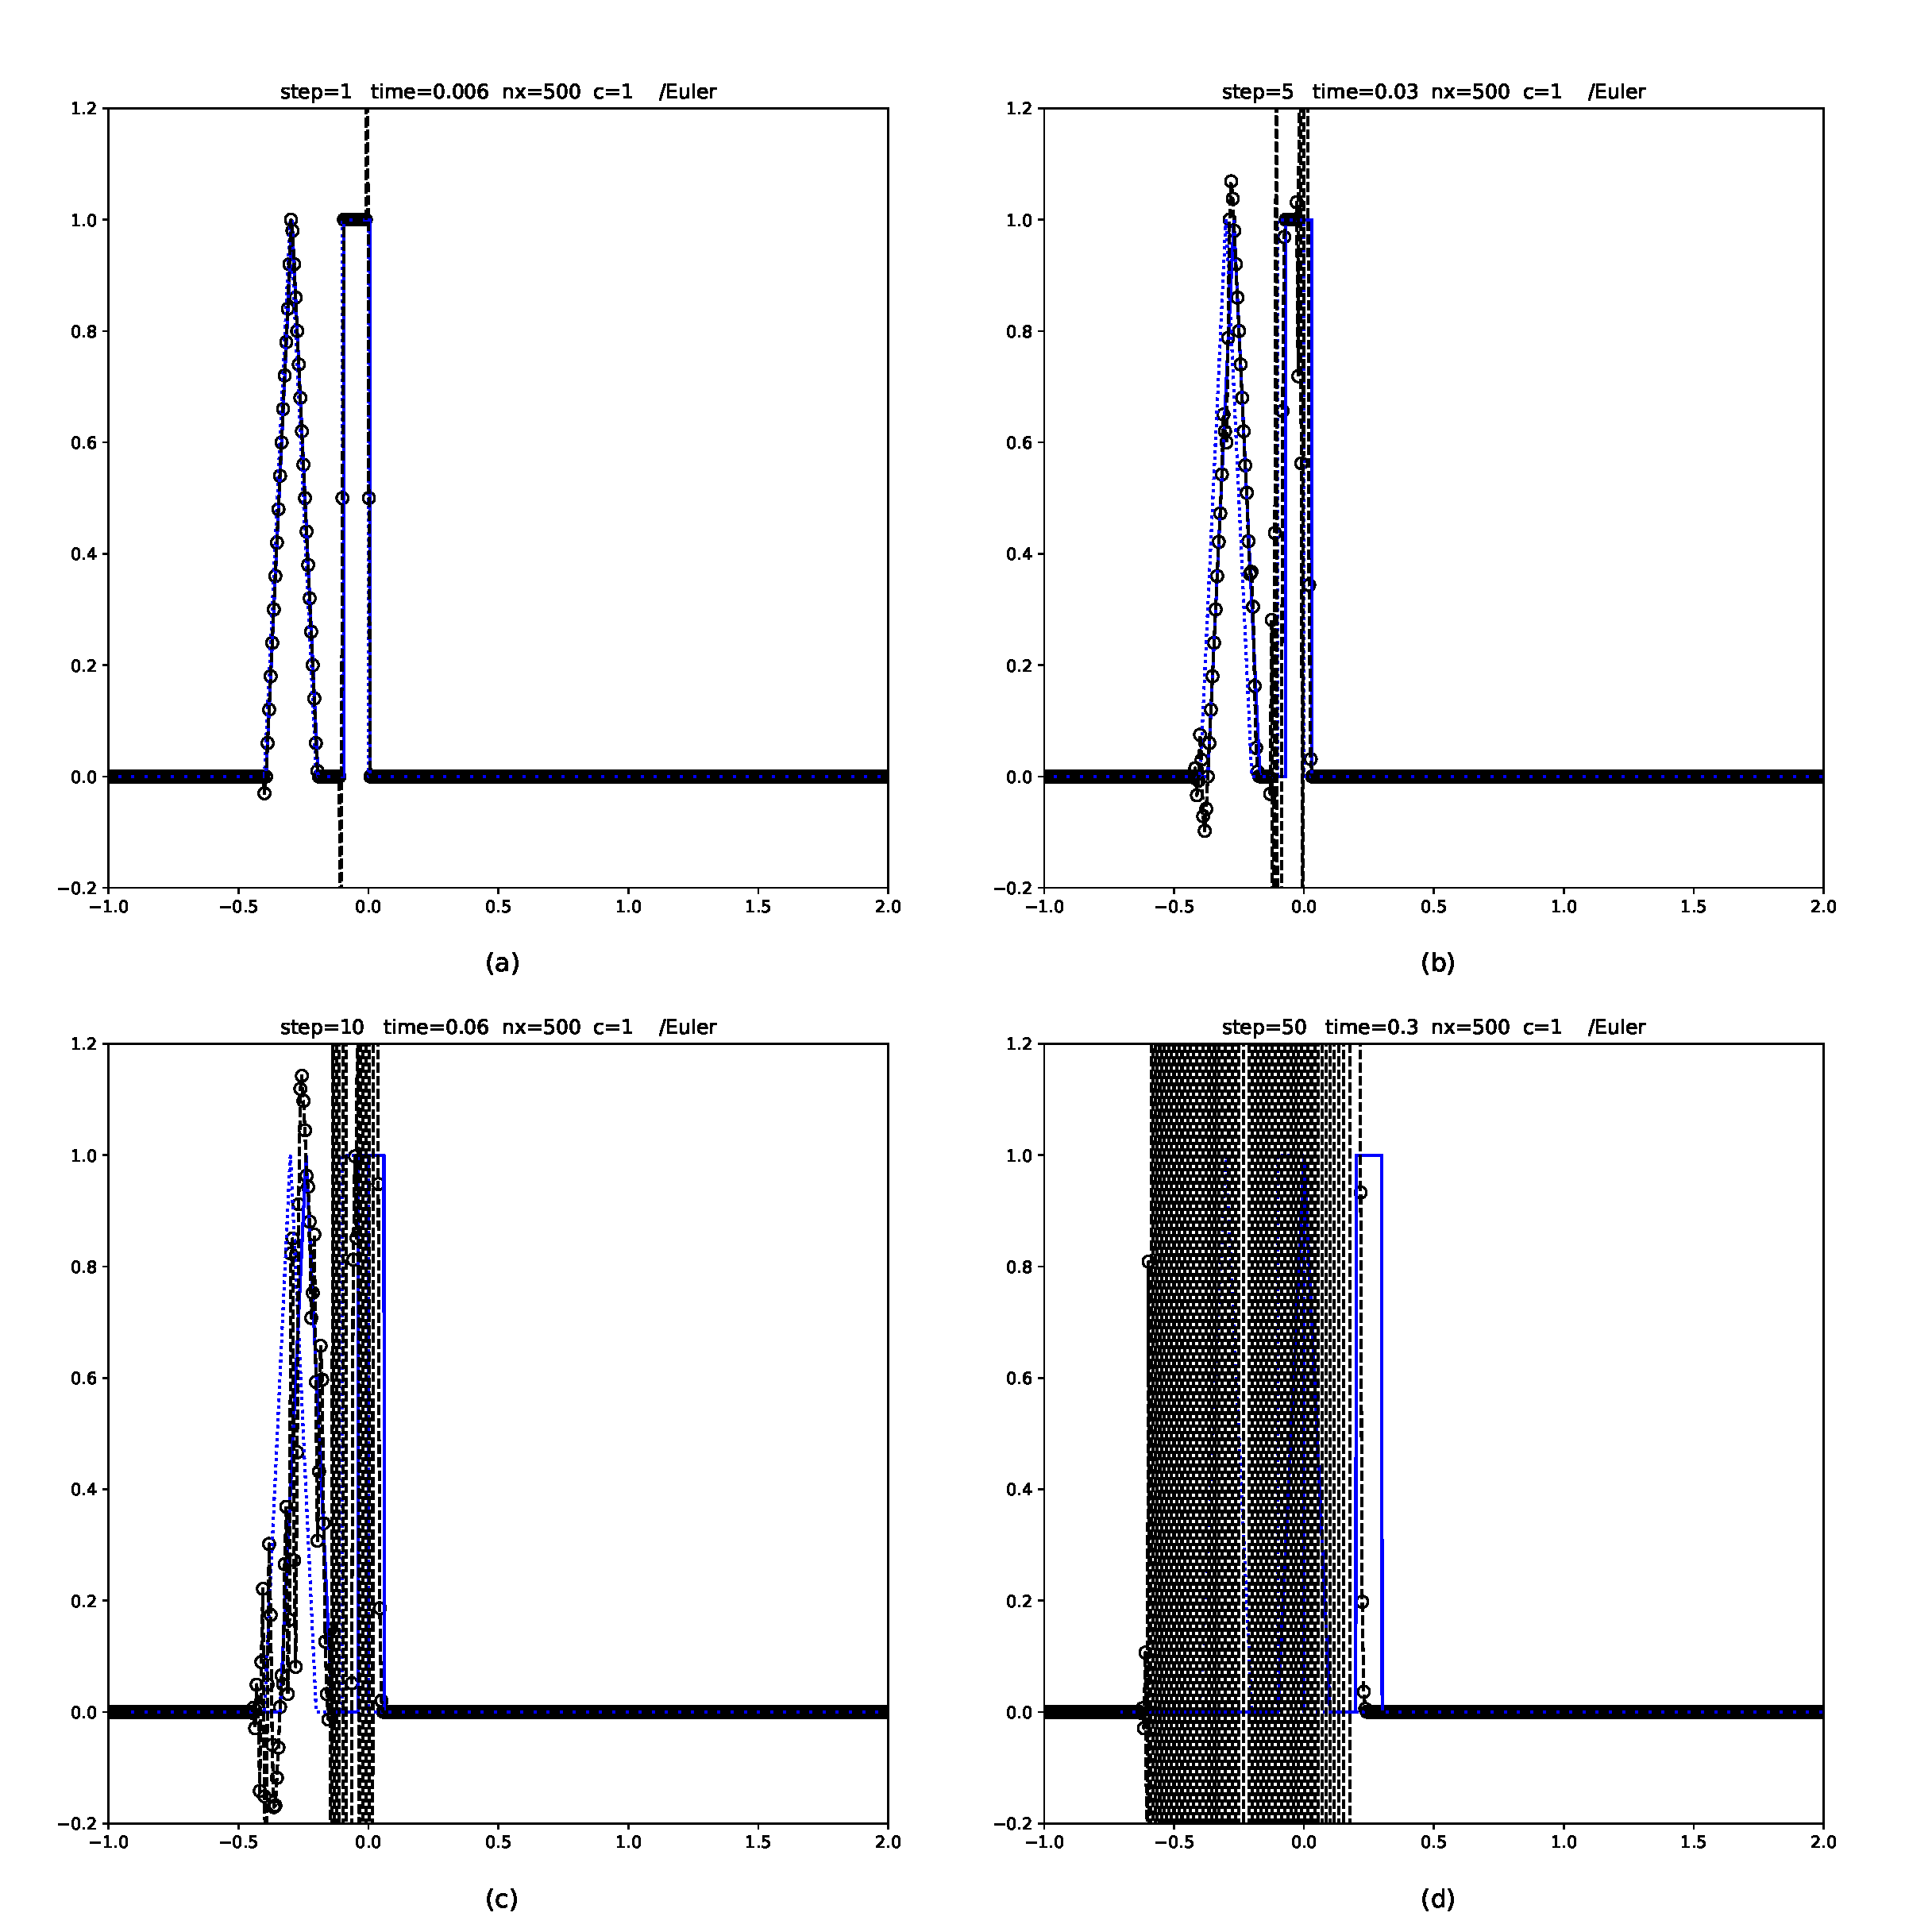
\includegraphics[width=\textwidth]{hw2_1_euler.eps}
	\caption{方程(\ref{EqnCon})在不稳定格式下的解. 其中虚线表示数值Euler格式的计算结果, 线上的圆圈表示具体网格上的数据. 同一时刻的精确解用实线表示. 作为对照, 初始时刻的值以点线表示, 坐标网格总数为500, $C = 1.0$. (a) Euler格式, $step = 1$, (b)  Euler格式, $step = 5$, (c)  Euler格式, $step = 10$, (d) Euler格式, $step = 50$.} \label{fig14}
\end{figure}

\section{Burgers方程}
已知初值为
\begin{align}
u|_{t=0} = \left\{\begin{array}{ll} 1.8, & x < -0.8,
\\
1.4 + 0.4 \cos\left[2 \pi (x + 0.8) \right], & -0.8 \le x < -0.3,
\\
1.0, & -0.3 \le x < 0.0,
\\
1.8, & x \ge 0.0
\end{array} \right.
\end{align}
在这个初值条件下, 本工作将设计两种差分格式, 分析Burgers方程
\begin{align}
\frac{\partial u}{\partial t} + u \frac{\partial u}{\partial x} = 0, \label{EqnBurgers}
\end{align}
的数值解, 并分析讨论数值计算结果. 
\subsection{Minmod格式}
这个小节介绍以Minmod格式来进行数值计算试验的情况. 首先定义\citep{Zheng2019}
\begin{align}
\sigma^n_j=\text{minmod}(\frac{u^n_j-u^n_{j-1}}{\Delta x}, \frac{u^n_{j+1}-u^n_{j}}{\Delta x})
\end{align}
其中
\begin{align}
\text{minmod}(a, b) = \left\{\begin{array}{ll} a, & \text{if\quad} |a|<|b| \text{\quad and\quad} ab>0,
\\
b, & \text{if\quad} |b|<|a| \text{\quad and\quad} ab>0,
\\
0, & \text{if\quad} ab\le 0.
\end{array} \right.
\end{align}
具体的, 方程(\ref{EqnBurgers})的Minmod计算格式为
\begin{align}
\begin{aligned}
u^{n+1}_j=u^{n}_j-&\frac{\Delta t}{\Delta x}(F(u^n_j)-F(u^n_{j-1}))+\\
&\frac{1}{2}\frac{\Delta t}{\Delta x}u^n_{j+1/2}(\Delta x-u^n_{j-1}\Delta t)(\sigma^n_j-\sigma^n_{j-1})
\end{aligned}	\label{minmod}
\end{align}
其中, $F(u)=\frac{1}{2}u^2$, $u^n_{j+1/2}=\frac{u^n_{j}+u^n_{j-1}}{2}$.

图\ref{BurgersM}是方程(\ref{EqnBurgers})的Minmod格式在时间$t = 0.25$, $0.5$, $0.75$, 和$1.0$的计算结果, 其中Courant系数取0.95, 即$\Delta t = 0.95 \frac{\Delta x}{\max(u)}$.
\subsection{Lax-Wendroff格式}
这个小节介绍以Lax-Wendroff格式对方程(\ref{EqnBurgers})进行数值计算试验的情况. 具体的计算格式为
\begin{align}
\begin{aligned}
u^{n+1}_j=&u^{n}_j-\frac{\Delta t}{\Delta x}\frac{F(u^n_{j+1})-F(u^n_{j-1})}{2}+\\
&\frac{1}{2}(\frac{\Delta t}{\Delta x})^2[u^n_{j+1/2}(F(u^n_{j+1})-F(u^n_j))-u^n_{j-1/2}(F(u^n_j)-F(u^n_{j-1}))]
%0.5*c^2*((u[j+1,n]+u[j,n])^2*(u[j+1,n]-u[j,n])/4-(u[j,n]+u[j-1,n])^2*(u[j,n]-u[j-1,n])/4)
\end{aligned}
\end{align}
其中, $F(u)=\frac{1}{2}u^2$.

图\ref{BurgersL}是方程(\ref{EqnBurgers})的Lax-Wendroff格式在时间$t = 0.25$, $0.5$, $0.75$, 和$1.0$的计算结果, 其中Courant系数取0.95, 即$\Delta t = 0.95 \frac{\Delta x}{\max(u)}$. 可以清楚的看到, 采用Lax-Wendroff格式得到的数值解会出现色散(即图\ref{BurgersL}出现的上冲和下冲)
\begin{figure}[htb]
	\begin{center}
		\begin{tabular}{cc}
			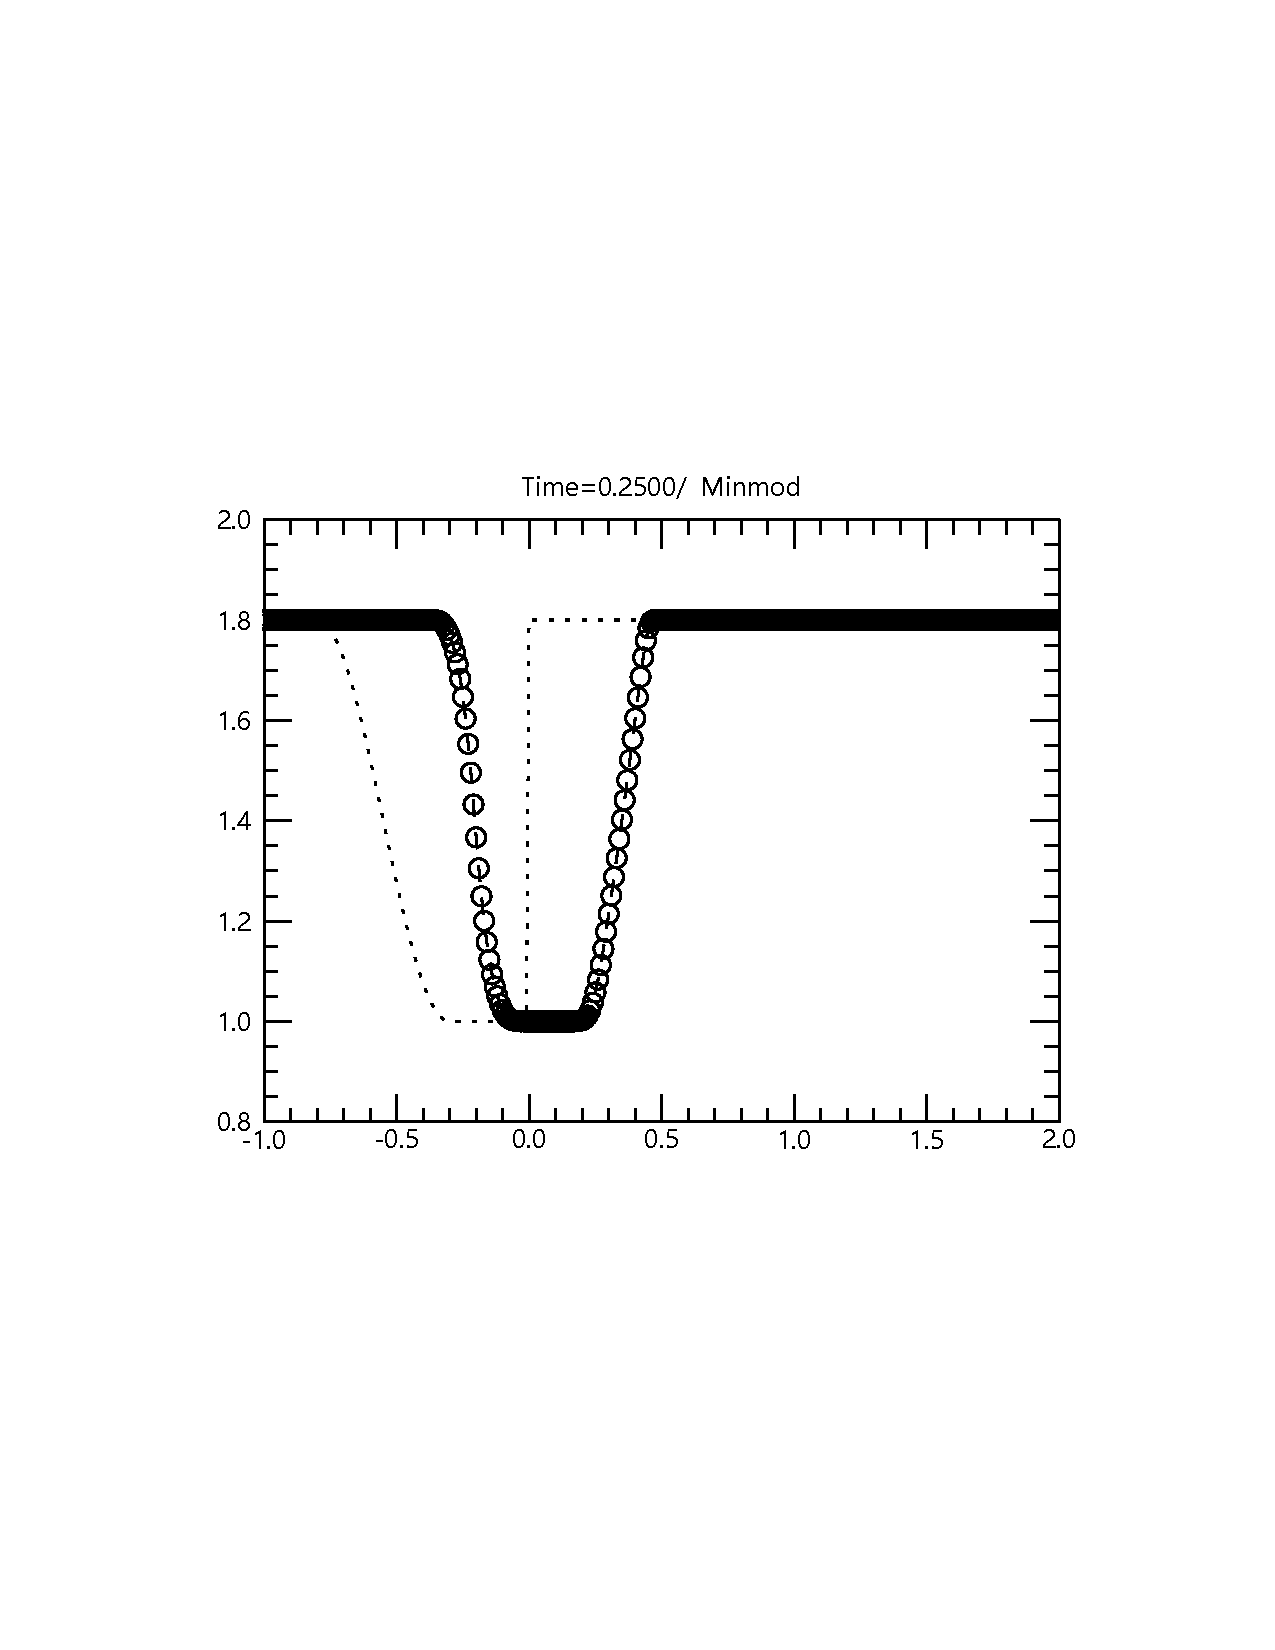
\includegraphics[width=.45\textwidth]{fig2_1_1}
			&
			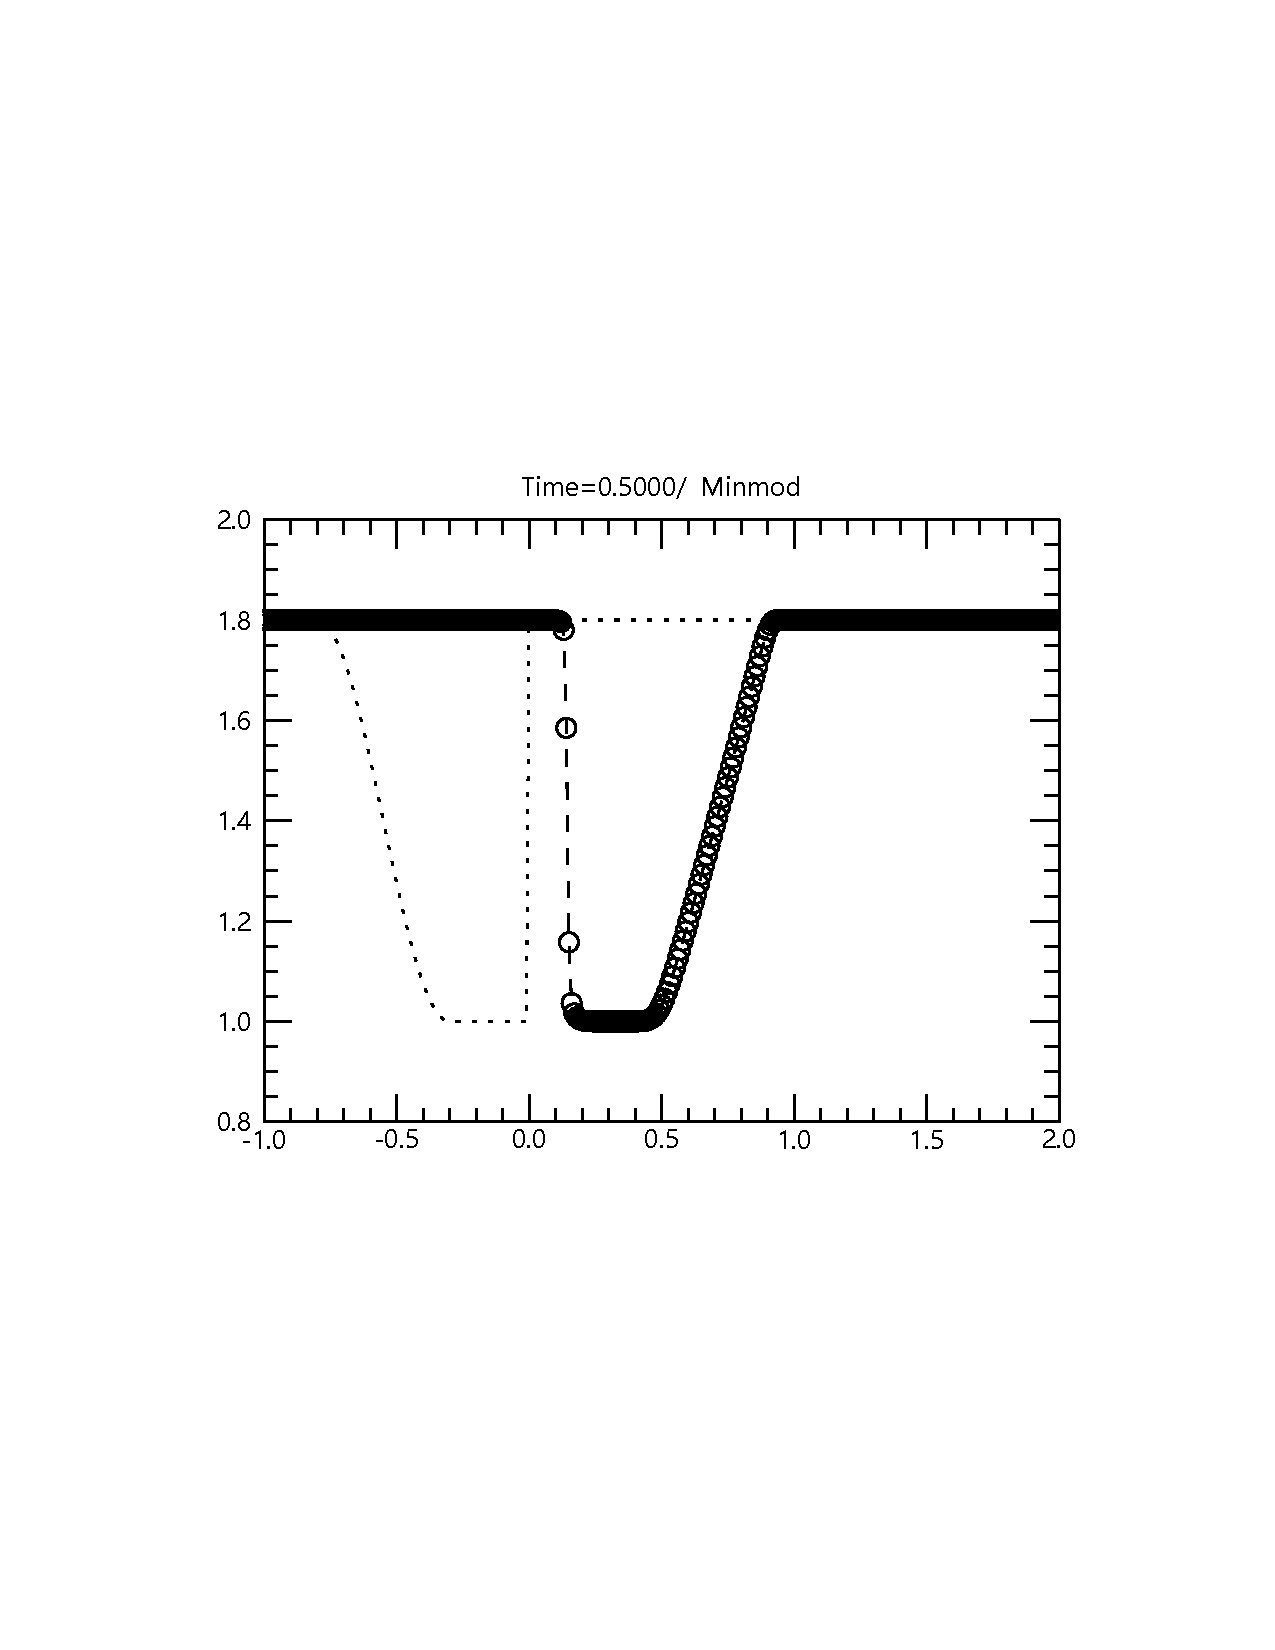
\includegraphics[width=.45\textwidth]{fig2_1_2}
			\\[-10pt]
			(a) & (b)
			\\
			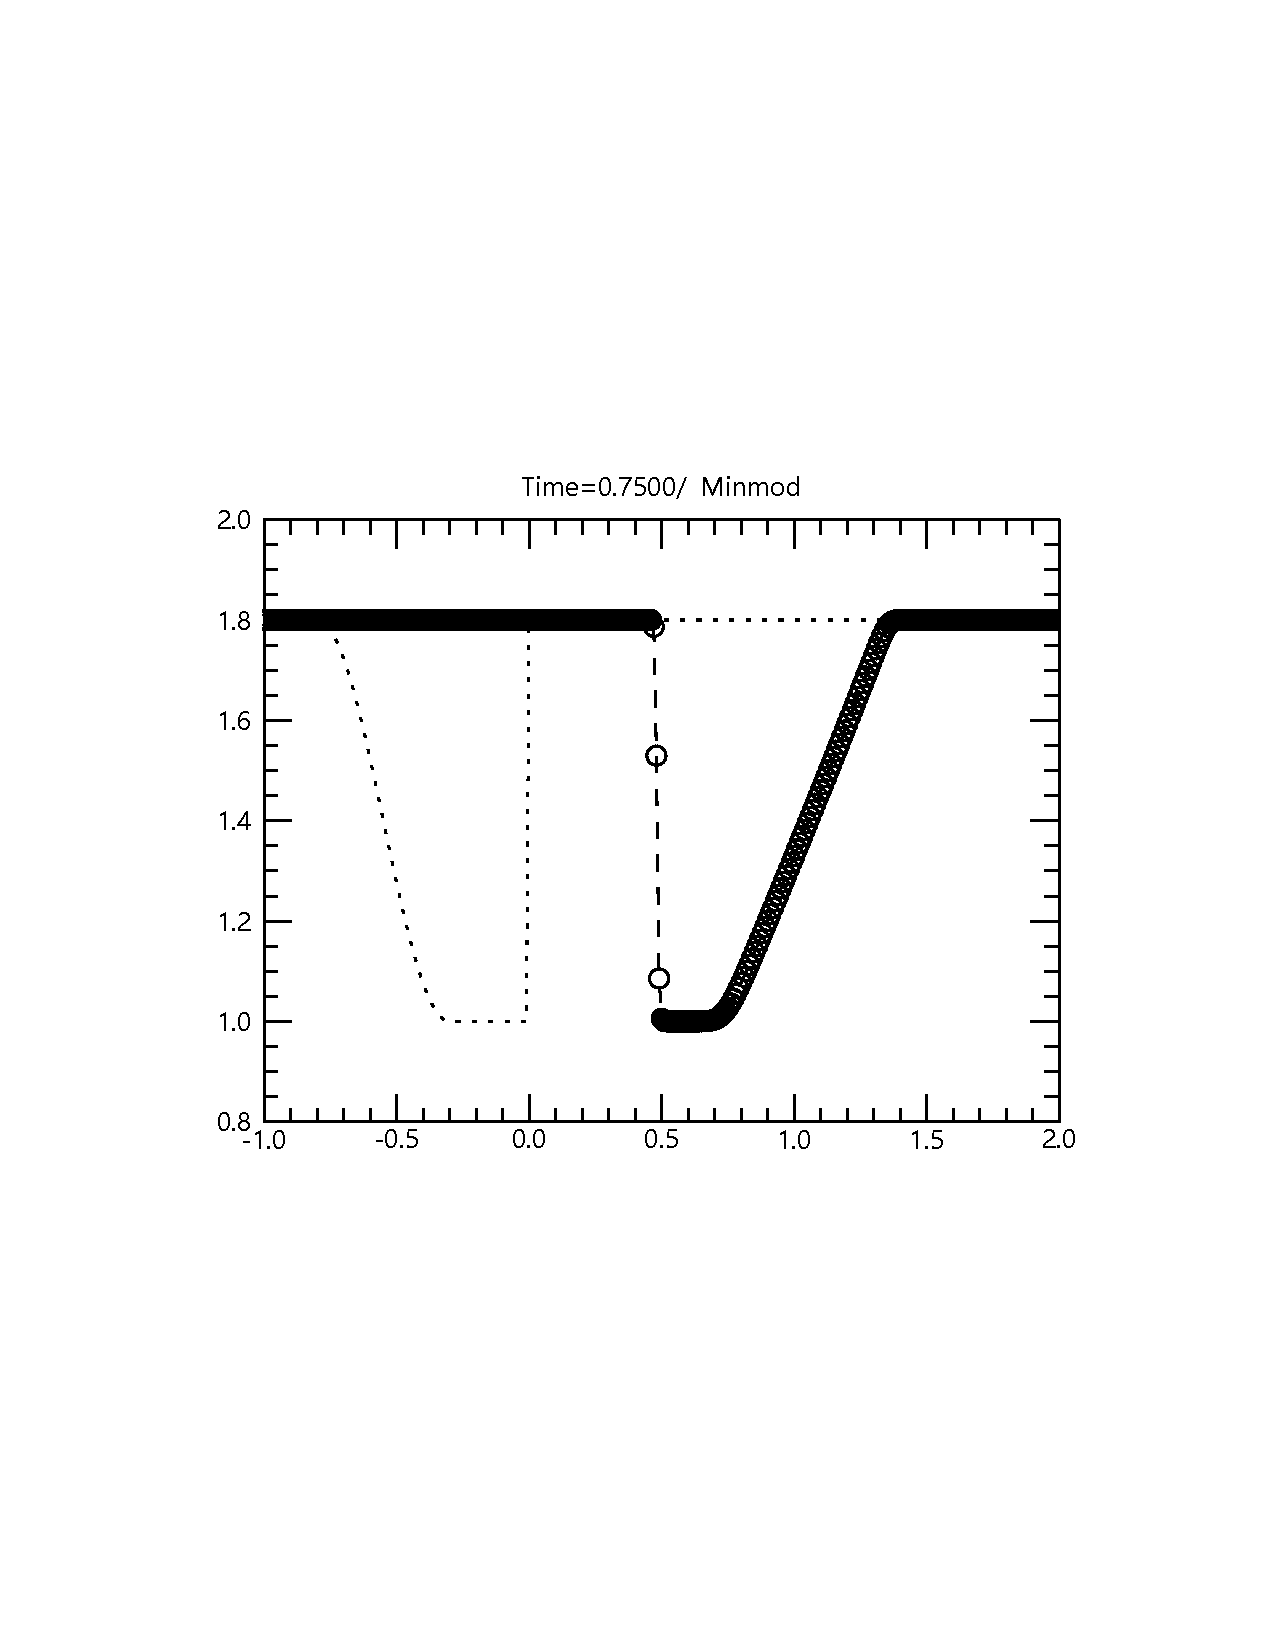
\includegraphics[width=.45\textwidth]{fig2_1_3}
			&
			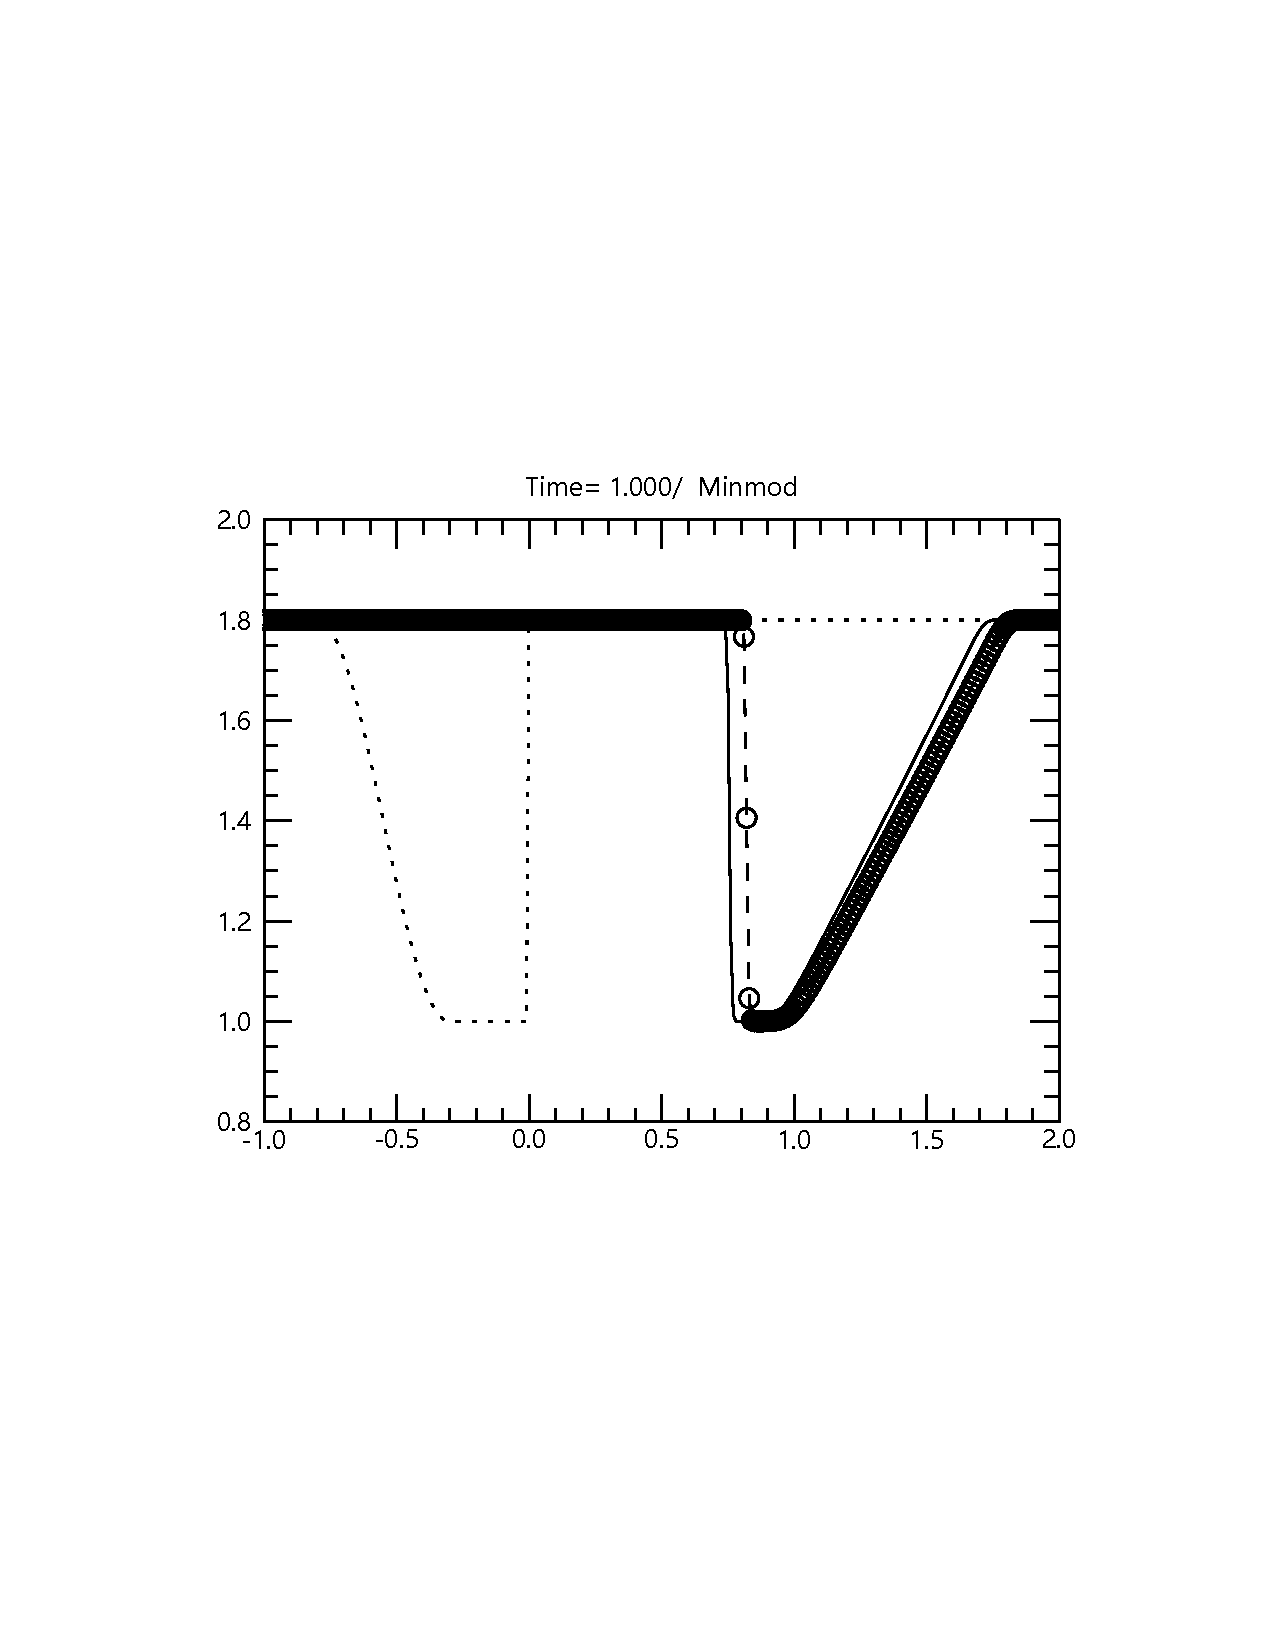
\includegraphics[width=.45\textwidth]{fig2_1_4}
			\\[-10pt]
			(c) & (d)
		\end{tabular}
	\end{center}
	\caption{%
		方程(\ref{EqnBurgers})的Minmode格式计算结果, 参数$x$从$-1.0$到$2.0$均匀分割, 取了301个点, Courant系数$C$取为0.95. 虚线表示数值格式的计算结果, 其中上面的圆圈表示具体的数据; 初始时刻的值以点线表示. (a) $t=0.25$, (b) $t=0.5$, (c) $t=0.75$, (d) $t=1.0$.
	}
	\label{BurgersM}
\end{figure}


\begin{figure}[htb]
	\begin{center}
		\begin{tabular}{cc}
			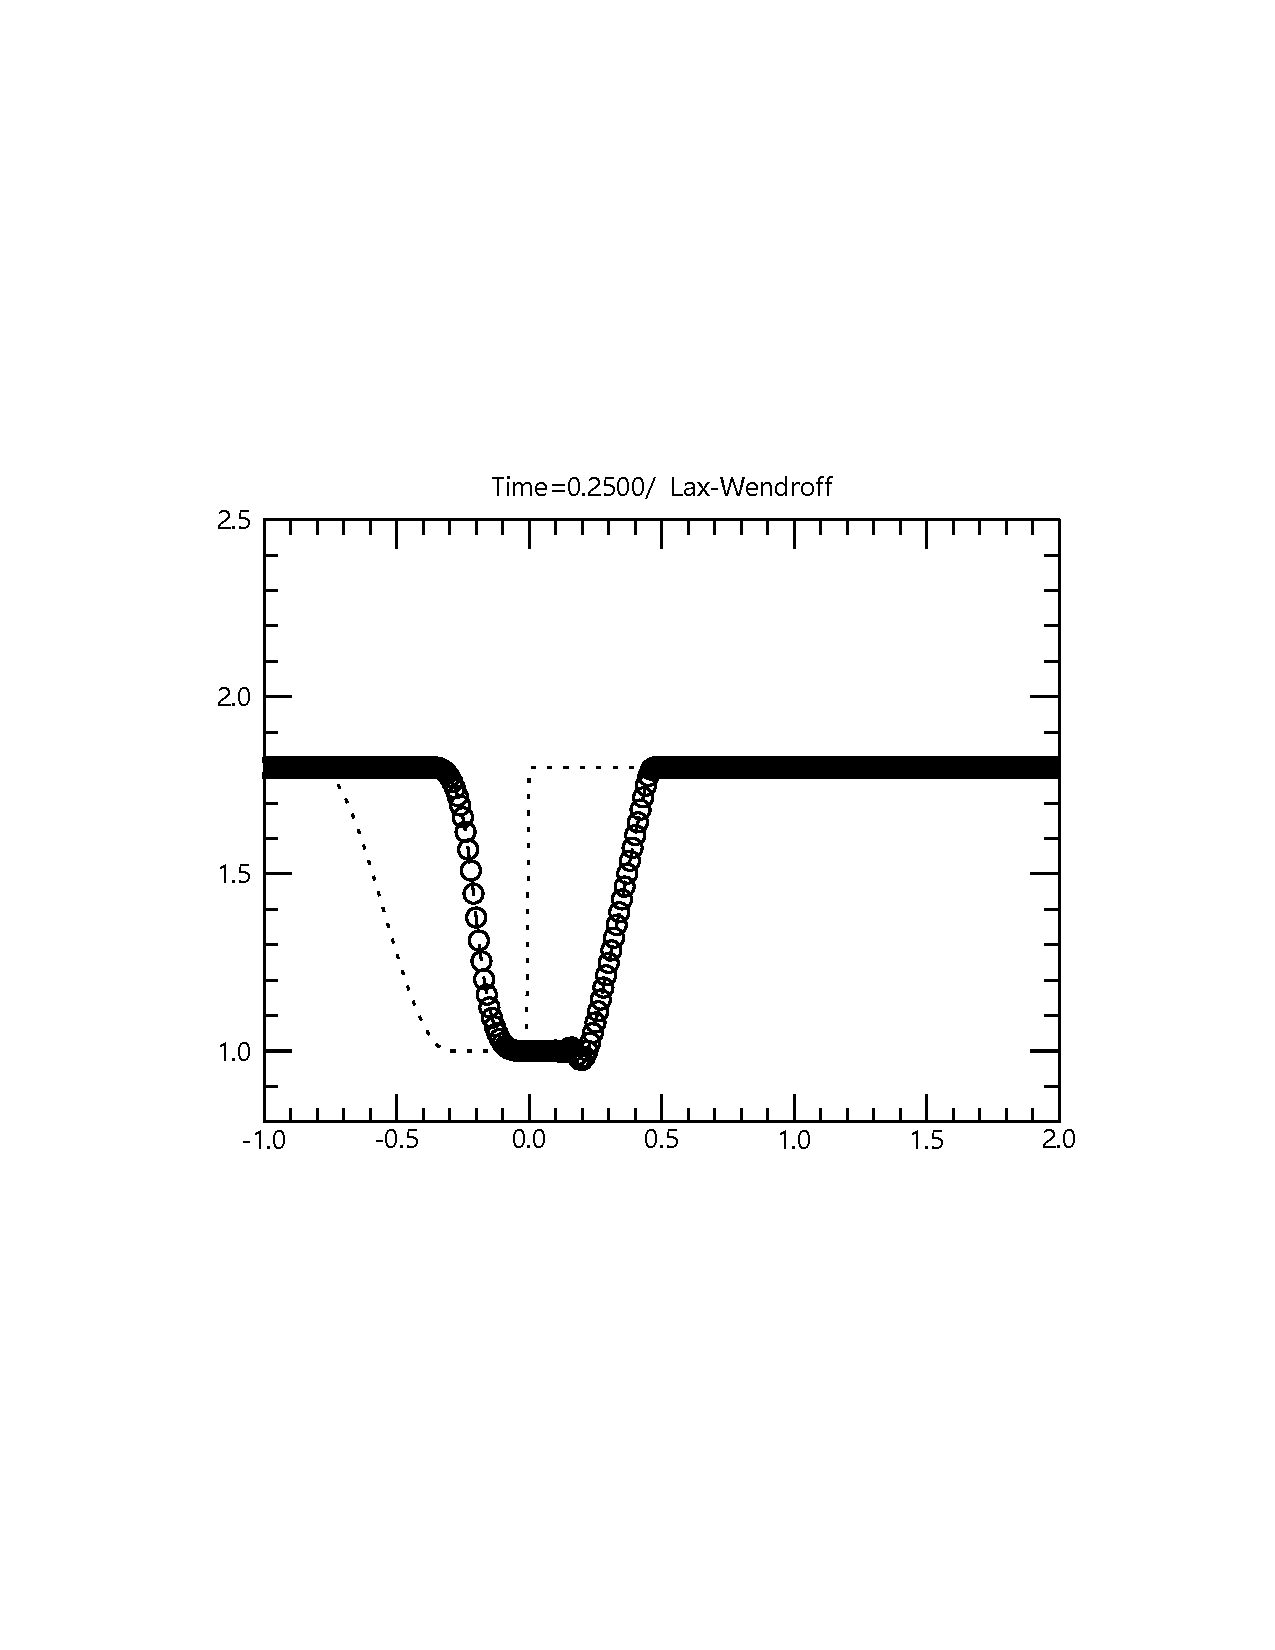
\includegraphics[width=.45\textwidth]{fig2_2_1}
			&
			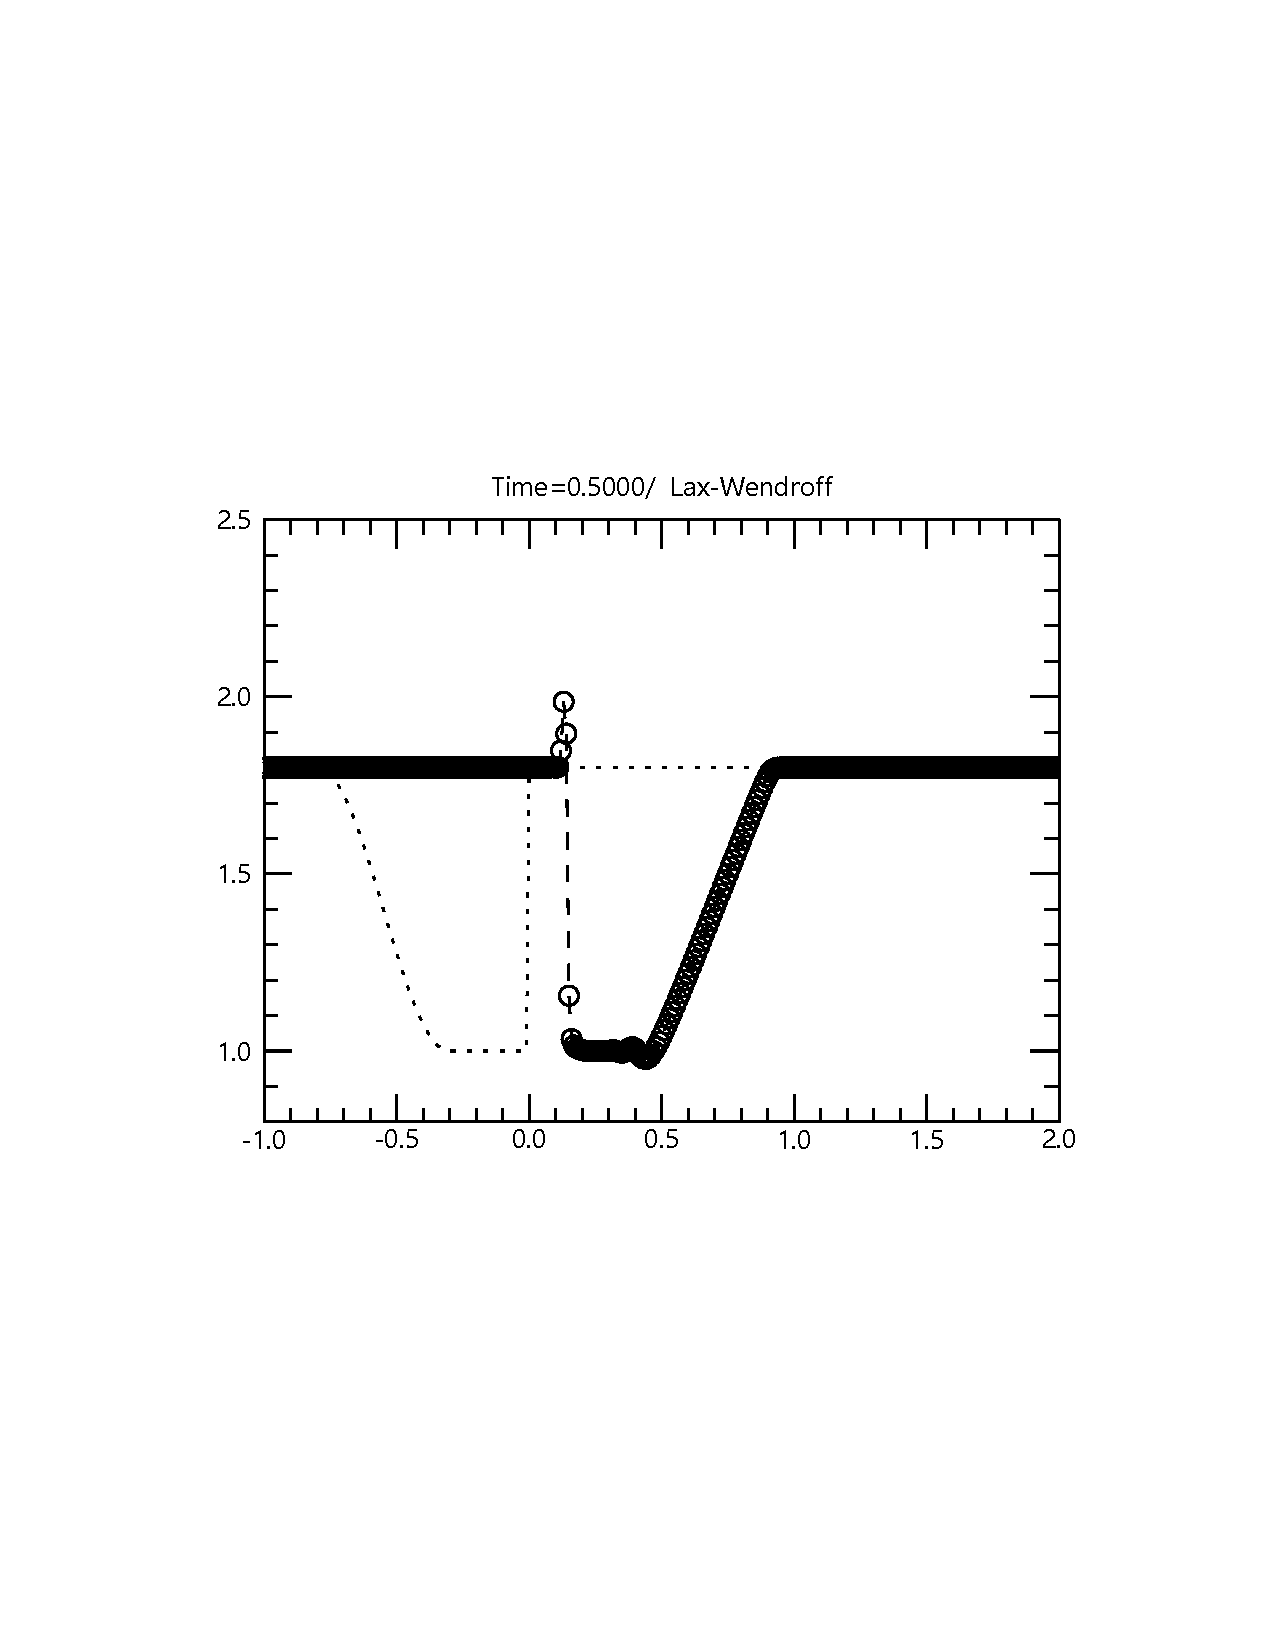
\includegraphics[width=.45\textwidth]{fig2_2_2}
			\\[-10pt]
			(a) & (b)
			\\
			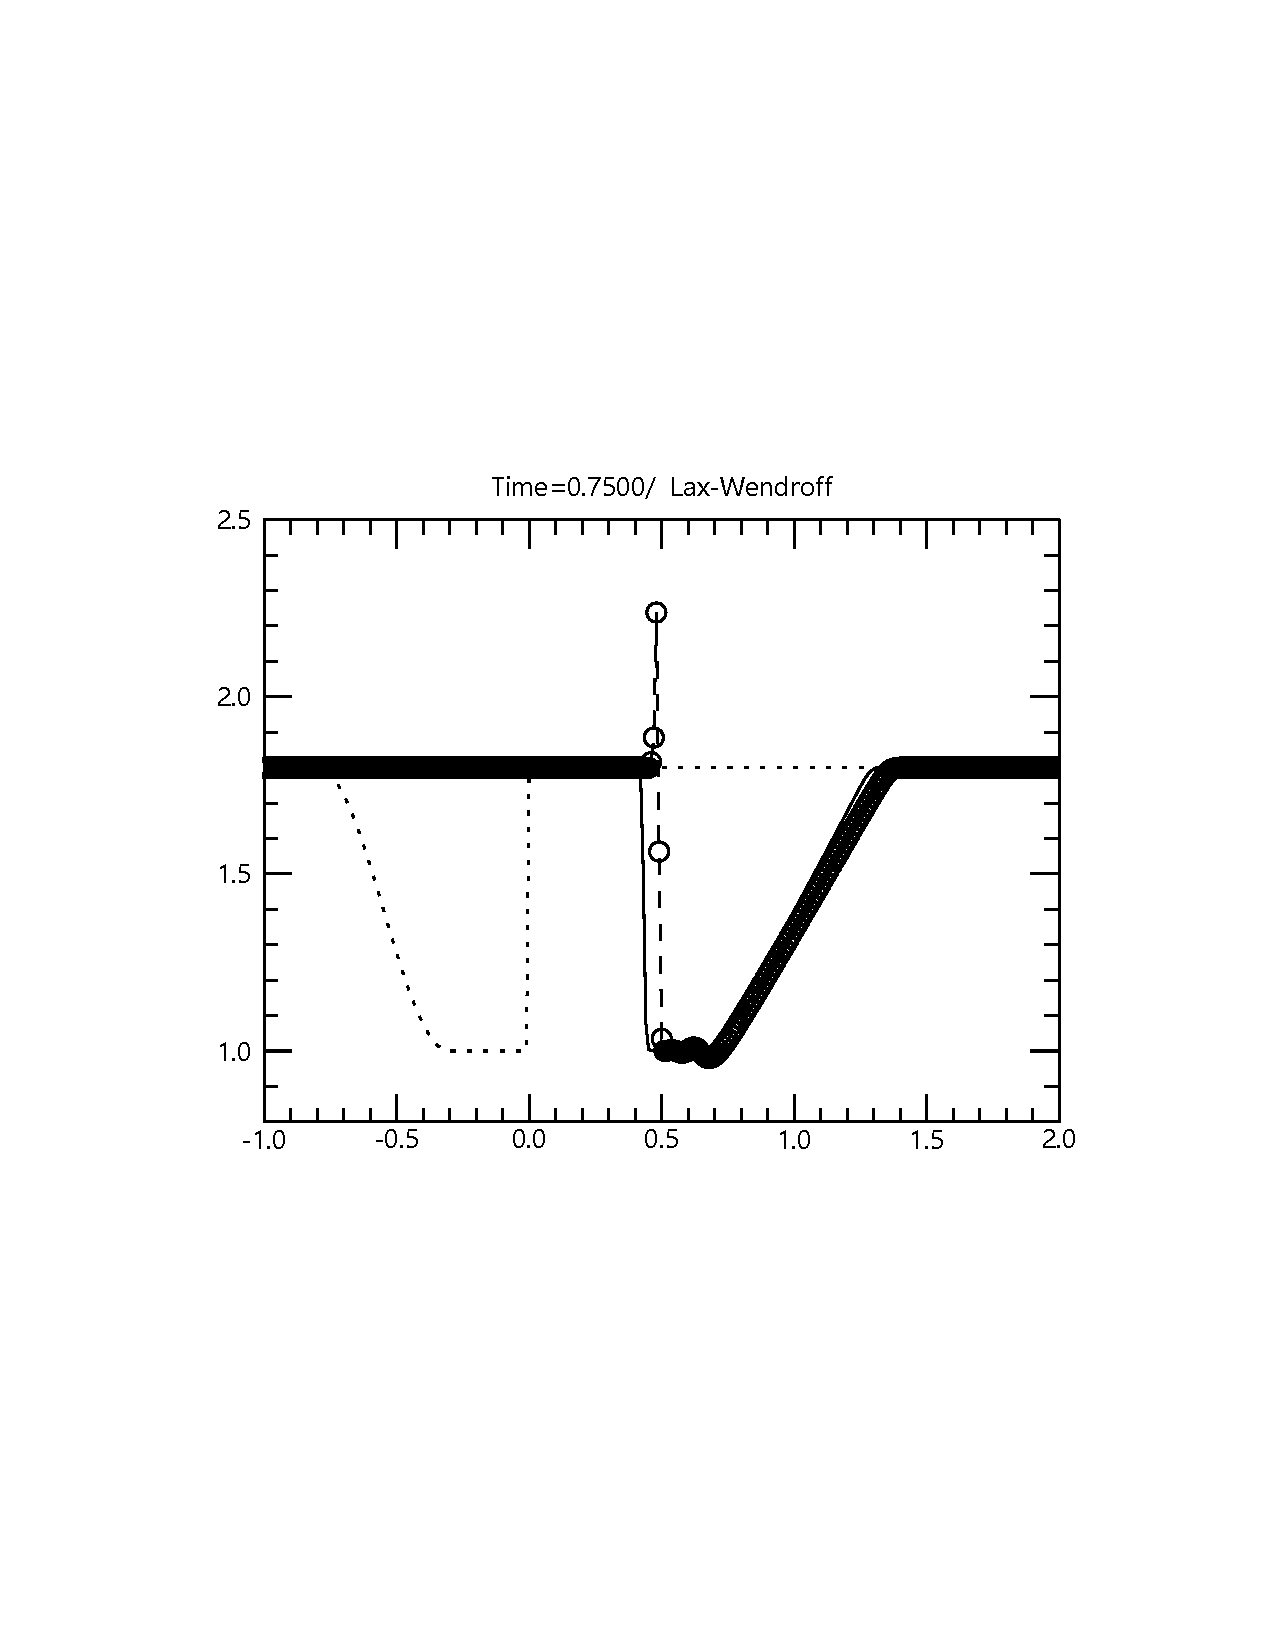
\includegraphics[width=.45\textwidth]{fig2_2_3}
			&
			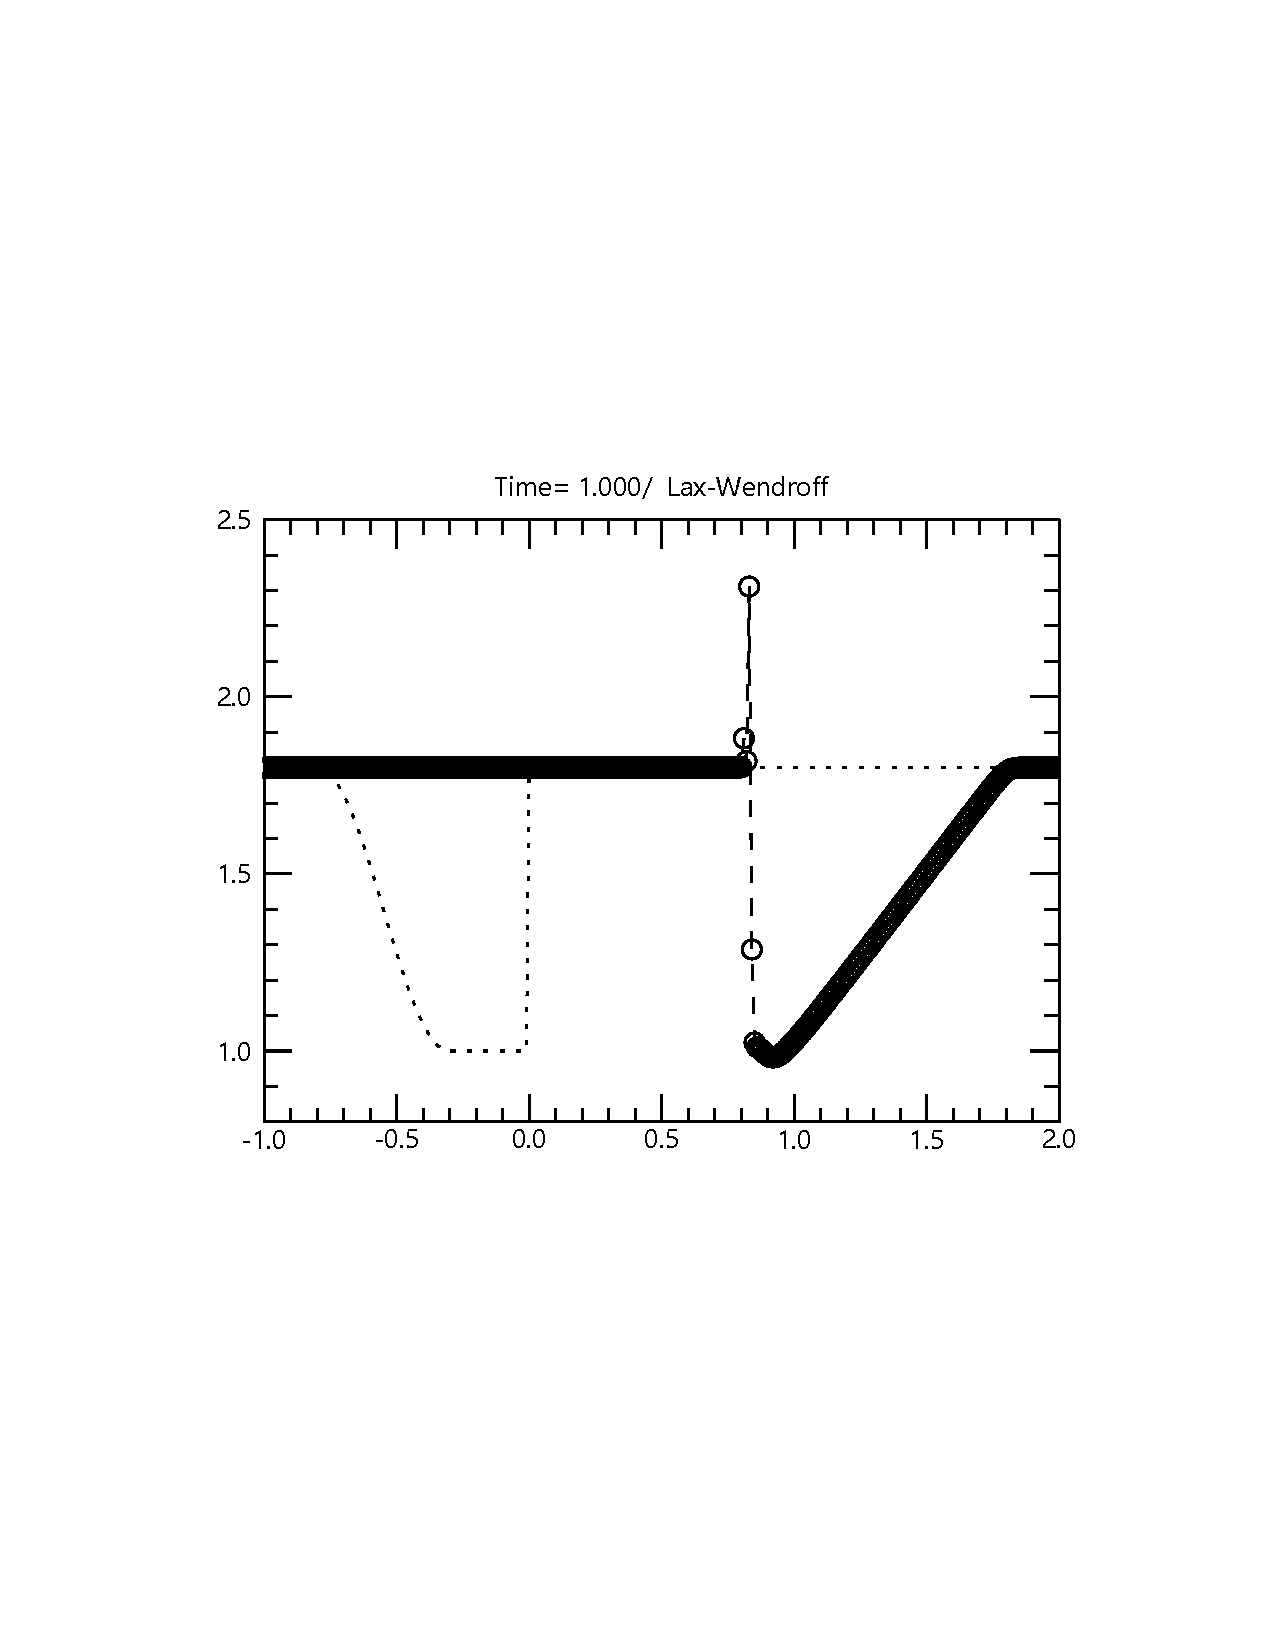
\includegraphics[width=.45\textwidth]{fig2_2_4}
			\\[-10pt]
			(c) & (d)
		\end{tabular}
	\end{center}
	\caption{%
		方程(\ref{EqnBurgers})的Lax-Wendroff格式计算结果, 参数$x$从-1.0到2.0均匀分割, 取了301个点, Courant系数$C$取为0.95. 虚线表示数值格式的计算结果, 其中上面的圆圈表示具体的数据; 初始时刻的值以点线表示. (a) $t=0.25$, (b) $t=0.5$, (c) $t=0.75$, (d) $t=1.0$.}
	\label{BurgersL}
\end{figure}

\section*{分工说明}

\begin{itemize}
	\item 毛东巍: 撰写报告;
	\item 张建: 完成第二节的内容;
	\item 钟志辉:完成第三节的内容.
\end{itemize}
特此说明: 以上分工仅以姓名拼音为序.
\section*{附件}

\begin{enumerate}
\item
assign2.tex--本报告的\LaTeX 文件
\item
assign2.pdf--本报告的PDF输出文件
\item
References.bib - 文献文件
\item 
hw2\_1.py--文中第二节所用的Python计算和图形绘制程序
\item
hw2\_2.pro--文中第三节图所用的IDL计算和图形绘制程序
\item
use\_hw2\_2.pro--文中第三节图所用的IDL计算和图形绘制程序
\item
hw2\_1\_c.eps - 行波方程(\ref{EqnCon})的不同格式数值计算结果, 对应图\ref{fig11}
\item
hw2\_1\_nx.eps - 行波方程(\ref{EqnCon})的不同网格数数值计算结果, 对应图\ref{fig12}
\item
hw2\_1\_time.eps - 行波方程(\ref{EqnCon})的不同时间数值计算结果, 对应图\ref{fig13}
\item
hw2\_1\_euler.eps - 行波方程(\ref{EqnCon})的Euler格式数值计算结果, 对应图\ref{fig14}

\item
fig2\_1\_1.pdf - Burgers方程(\ref{EqnBurgers})在Minmod格式下的数值计算结果, 对应图\ref{BurgersM}(a)
\item
fig2\_1\_2.pdf - Burgers方程(\ref{EqnBurgers})在Minmod格式下的数值计算结果, 对应图\ref{BurgersM}(b)
\item
fig2\_1\_3.pdf - Burgers方程(\ref{EqnBurgers})在Minmod格式下的数值计算结果, 对应图\ref{BurgersM}(c)
\item
fig2\_1\_4.pdf - Burgers方程(\ref{EqnBurgers})在Minmod格式下的数值计算结果, 对应图\ref{BurgersM}(d)
\item
fig2\_2\_1.pdf - Burgers方程(\ref{EqnBurgers})在Lax-Windroff格式下的数值计算结果, 对应图\ref{BurgersL}(a)
\item
fig2\_2\_2.pdf - Burgers方程(\ref{EqnBurgers})在Lax-Windroff格式下的数值计算结果, 对应图\ref{BurgersL}(b)
\item
fig2\_2\_3.pdf - Burgers方程(\ref{EqnBurgers})在Lax-Windroff格式下的数值计算结果, 对应图\ref{BurgersL}(c)
\item
fig2\_2\_4.pdf - Burgers方程(\ref{EqnBurgers})在Lax-Windroff格式下的数值计算结果, 对应图\ref{BurgersL}(d)
\end{enumerate}



\bibliographystyle{apalike}
\bibliography{References}

\end{document}
